%!TEX encoding = UTF-8 Unicode

\documentclass[landscape]{book}
\usepackage[a3paper]{geometry}

\usepackage{verbatim}

\usepackage{hyperref}

\usepackage{tikz}

\usetikzlibrary{
  arrows,
  shapes.misc,% wg. rounded rectangle
  shapes.arrows,%
  matrix,%
  scopes,%
  shadows%
}

\tikzset{
  nonterminal/.style={
    % The shape:
    rectangle,
    % The size:
    minimum size=6mm,
    % The border:
    very thick,
    draw=red!50!black!50,         % 50% red and 50% black,
                                  % and that mixed with 50% white
    % The filling:
    top color=white,              % a shading that is white at the top...
    bottom color=red!50!black!20, % and something else at the bottom
    % Font
    font=\itshape\small
  },
  terminal/.style={
    % The shape:
    rounded rectangle,
    minimum size=6mm,
    % The rest
    very thick,draw=black!50,
    top color=white,bottom color=black!20,
    font=\ttfamily\small
  },
  firstPoint/.style={circle,>=stealth',thick,draw=black!50},
  point/.style={coordinate,>=stealth',thick,draw=black!50},
  tip/.style={->,shorten >=0.007pt},
  lastPoint/.style={rectangle,>=stealth',thick,draw=black!50},
  every join/.style={rounded corners}
}

\newcommand\nonTerminalSection[2]{\section{Nonterminal \texttt{#1}}\label{nt:#2}}
\newcommand\ruleSubsection[3]{\subsection{Component \texttt{#1}, in file \texttt{#2}, line #3}}
\newcommand\ruleMatrixColumnSeparation{3mm}
\newcommand\ruleMatrixRowSeparation{3mm}
\newcommand\nonTerminalSymbol[2]{\hyperref[nt:#2]{#1}}
\newcommand\startSymbol[2]{The start symbol is \hyperref[nt:#2]{#1}.}

\newcommand\nonTerminalSummaryStart{This is the alphabetical list of non terminal : }
\newcommand\nonTerminalSummary[2]{\hyperref[nt:#2]{#1}}
\newcommand\nonTerminalSummarySeparator{, }
\newcommand\nonTerminalSummaryEnd{.\\}

\begin{document}

\title{\Huge{Grammar \texttt{gtl\_grammar}}}
\date \today 

\maketitle

\startSymbol{gtl\_start\_symbol}{6}

\nonTerminalSummaryStart \nonTerminalSummary{gtl\_argument\_list}{5}\nonTerminalSummarySeparator \nonTerminalSummary{gtl\_expression}{0}\nonTerminalSummarySeparator \nonTerminalSummary{gtl\_factor}{14}\nonTerminalSummarySeparator \nonTerminalSummary{gtl\_file\_name}{9}\nonTerminalSummarySeparator \nonTerminalSummary{gtl\_import}{3}\nonTerminalSummarySeparator \nonTerminalSummary{gtl\_relation\_factor}{11}\nonTerminalSummarySeparator \nonTerminalSummary{gtl\_relation\_term}{10}\nonTerminalSummarySeparator \nonTerminalSummary{gtl\_simple\_expression}{12}\nonTerminalSummarySeparator \nonTerminalSummary{gtl\_simple\_instruction}{4}\nonTerminalSummarySeparator \nonTerminalSummary{gtl\_sorting\_order}{15}\nonTerminalSummarySeparator \nonTerminalSummary{gtl\_start\_symbol}{6}\nonTerminalSummarySeparator \nonTerminalSummary{gtl\_template\_instruction}{8}\nonTerminalSummarySeparator \nonTerminalSummary{gtl\_template\_instruction\_list}{7}\nonTerminalSummarySeparator \nonTerminalSummary{gtl\_term}{13}\nonTerminalSummarySeparator \nonTerminalSummary{gtl\_variable}{1}\nonTerminalSummarySeparator \nonTerminalSummary{gtl\_variable\_or\_here}{2}\nonTerminalSummaryEnd \nonTerminalSection{gtl\_argument\_list}{5}

\ruleSubsection{gtl\_expression\_parser}{gtl\_expression\_parser}{736}

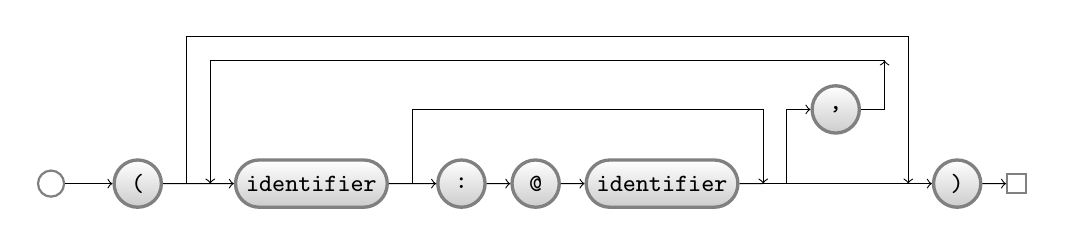
\begin{tikzpicture}
  \matrix[column sep=\ruleMatrixColumnSeparation, row sep=\ruleMatrixRowSeparation] {
    & & & & \node (p3-4) [point] {}; & \\
    & & & & & & & & & & & & & \node (p2-13) [point] {}; & \\
    & & & & & & & \node (p1-7) [point] {}; & & & & & \node (p1-12) [terminal] {,}; & \\
    \node (P0start) [firstPoint] {}; & & \node (p0-2) [terminal] {(}; & \node (p0-3) [point] {}; & \node (p0-4) [point] {}; & \node (p0-5) [terminal] {identifier}; & \node (p0-6) [point] {}; & \node (p0-7) [terminal] {:}; & \node (p0-8) [terminal] {@}; & \node (p0-9) [terminal] {identifier}; & \node (p0-10) [point] {}; & \node (p0-11) [point] {}; & & & \node (p0-14) [point] {}; & \node (p0-15) [terminal] {)}; & \node (p0-16) [lastPoint] {}; & \\
  };
  \draw[->] (P0start) -- (p0-2) ;
  \draw[->] (p0-2) -- (p0-5) ;
  \draw[->] (p0-5) -- (p0-7) ;
  \draw[->] (p0-7) -- (p0-8) ;
  \draw[->] (p0-8) -- (p0-9) ;
  \draw (p0-6) |- (p1-7) ;
  \draw (p0-9) -- (p0-10) ;
  \draw[->] (p1-7) -| (p0-10) ;
  \draw[->] (p0-11) |- (p1-12) ;
  \draw[->] (p2-13) -| (p0-4) ;
  \draw[->] (p1-12) -| (p2-13) ;
  \draw (p0-3) |- (p3-4) ;
  \draw (p0-10) -- (p0-14) ;
  \draw[->] (p3-4) -| (p0-14) ;
  \draw[->] (p0-14) -- (p0-15) ;
  \draw[->] (p0-15) -- (p0-16) ;
\end{tikzpicture}

\nonTerminalSection{gtl\_expression}{0}

\ruleSubsection{gtl\_expression\_parser}{gtl\_expression\_parser}{33}

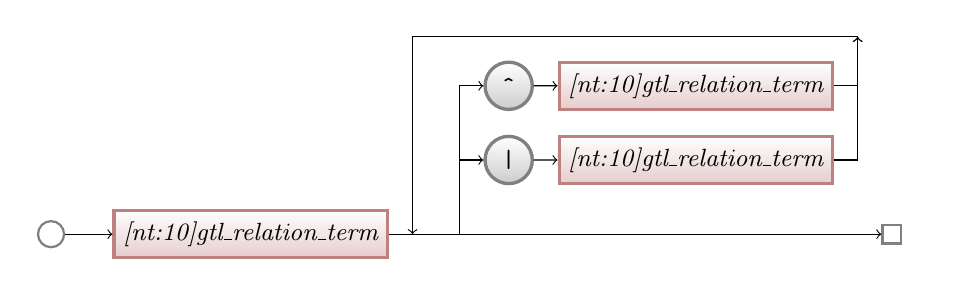
\begin{tikzpicture}
  \matrix[column sep=\ruleMatrixColumnSeparation, row sep=\ruleMatrixRowSeparation] {
    & & & & & & & & \node (p3-8) [point] {}; & \\
    & & & & & & \node (p2-6) [terminal] {\verb=^=}; & \node (p2-7) [nonterminal] {\nonTerminalSymbol{gtl\_relation\_term}{10}}; & \\
    & & & & & & \node (p1-6) [terminal] {|}; & \node (p1-7) [nonterminal] {\nonTerminalSymbol{gtl\_relation\_term}{10}}; & \\
    \node (P0start) [firstPoint] {}; & & \node (p0-2) [nonterminal] {\nonTerminalSymbol{gtl\_relation\_term}{10}}; & \node (p0-3) [point] {}; & \node (p0-4) [point] {}; & \node (p0-5) [point] {}; & & & & \node (p0-9) [lastPoint] {}; & \\
  };
  \draw[->] (P0start) -- (p0-2) ;
  \draw (p0-2) -- (p0-4) ;
  \draw[->] (p0-5) |- (p1-6) ;
  \draw[->] (p1-6) -- (p1-7) ;
  \draw[->] (p0-5) |- (p2-6) ;
  \draw[->] (p2-6) -- (p2-7) ;
  \draw[->] (p3-8) -| (p0-3) ;
  \draw[->] (p1-7) -| (p3-8) ;
  \draw[->] (p2-7) -| (p3-8) ;
  \draw[->] (p0-4) -- (p0-9) ;
\end{tikzpicture}

\nonTerminalSection{gtl\_factor}{14}

\ruleSubsection{gtl\_expression\_parser}{gtl\_expression\_parser}{192}

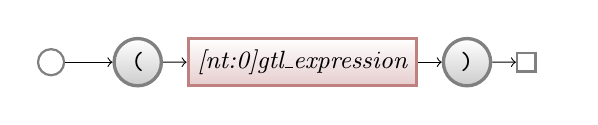
\begin{tikzpicture}
  \matrix[column sep=\ruleMatrixColumnSeparation, row sep=\ruleMatrixRowSeparation] {
    \node (P0start) [firstPoint] {}; & & \node (p0-2) [terminal] {(}; & \node (p0-3) [nonterminal] {\nonTerminalSymbol{gtl\_expression}{0}}; & \node (p0-4) [terminal] {)}; & \node (p0-5) [lastPoint] {}; & \\
  };
  \draw[->] (P0start) -- (p0-2) ;
  \draw[->] (p0-2) -- (p0-3) ;
  \draw[->] (p0-3) -- (p0-4) ;
  \draw[->] (p0-4) -- (p0-5) ;
\end{tikzpicture}

\ruleSubsection{gtl\_expression\_parser}{gtl\_expression\_parser}{208}

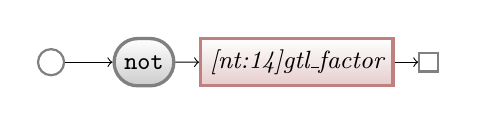
\begin{tikzpicture}
  \matrix[column sep=\ruleMatrixColumnSeparation, row sep=\ruleMatrixRowSeparation] {
    \node (P0start) [firstPoint] {}; & & \node (p0-2) [terminal] {not}; & \node (p0-3) [nonterminal] {\nonTerminalSymbol{gtl\_factor}{14}}; & \node (p0-4) [lastPoint] {}; & \\
  };
  \draw[->] (P0start) -- (p0-2) ;
  \draw[->] (p0-2) -- (p0-3) ;
  \draw[->] (p0-3) -- (p0-4) ;
\end{tikzpicture}

\ruleSubsection{gtl\_expression\_parser}{gtl\_expression\_parser}{220}

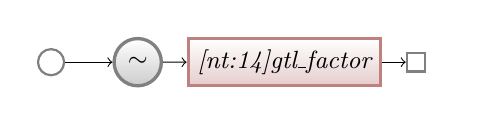
\begin{tikzpicture}
  \matrix[column sep=\ruleMatrixColumnSeparation, row sep=\ruleMatrixRowSeparation] {
    \node (P0start) [firstPoint] {}; & & \node (p0-2) [terminal] {$\sim$}; & \node (p0-3) [nonterminal] {\nonTerminalSymbol{gtl\_factor}{14}}; & \node (p0-4) [lastPoint] {}; & \\
  };
  \draw[->] (P0start) -- (p0-2) ;
  \draw[->] (p0-2) -- (p0-3) ;
  \draw[->] (p0-3) -- (p0-4) ;
\end{tikzpicture}

\ruleSubsection{gtl\_expression\_parser}{gtl\_expression\_parser}{232}

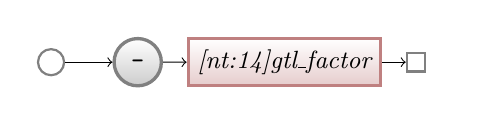
\begin{tikzpicture}
  \matrix[column sep=\ruleMatrixColumnSeparation, row sep=\ruleMatrixRowSeparation] {
    \node (P0start) [firstPoint] {}; & & \node (p0-2) [terminal] {-}; & \node (p0-3) [nonterminal] {\nonTerminalSymbol{gtl\_factor}{14}}; & \node (p0-4) [lastPoint] {}; & \\
  };
  \draw[->] (P0start) -- (p0-2) ;
  \draw[->] (p0-2) -- (p0-3) ;
  \draw[->] (p0-3) -- (p0-4) ;
\end{tikzpicture}

\ruleSubsection{gtl\_expression\_parser}{gtl\_expression\_parser}{244}

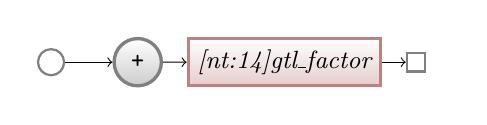
\begin{tikzpicture}
  \matrix[column sep=\ruleMatrixColumnSeparation, row sep=\ruleMatrixRowSeparation] {
    \node (P0start) [firstPoint] {}; & & \node (p0-2) [terminal] {+}; & \node (p0-3) [nonterminal] {\nonTerminalSymbol{gtl\_factor}{14}}; & \node (p0-4) [lastPoint] {}; & \\
  };
  \draw[->] (P0start) -- (p0-2) ;
  \draw[->] (p0-2) -- (p0-3) ;
  \draw[->] (p0-3) -- (p0-4) ;
\end{tikzpicture}

\ruleSubsection{gtl\_expression\_parser}{gtl\_expression\_parser}{256}

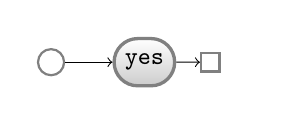
\begin{tikzpicture}
  \matrix[column sep=\ruleMatrixColumnSeparation, row sep=\ruleMatrixRowSeparation] {
    \node (P0start) [firstPoint] {}; & & \node (p0-2) [terminal] {yes}; & \node (p0-3) [lastPoint] {}; & \\
  };
  \draw[->] (P0start) -- (p0-2) ;
  \draw[->] (p0-2) -- (p0-3) ;
\end{tikzpicture}

\ruleSubsection{gtl\_expression\_parser}{gtl\_expression\_parser}{269}

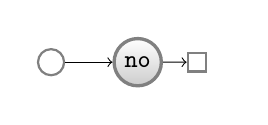
\begin{tikzpicture}
  \matrix[column sep=\ruleMatrixColumnSeparation, row sep=\ruleMatrixRowSeparation] {
    \node (P0start) [firstPoint] {}; & & \node (p0-2) [terminal] {no}; & \node (p0-3) [lastPoint] {}; & \\
  };
  \draw[->] (P0start) -- (p0-2) ;
  \draw[->] (p0-2) -- (p0-3) ;
\end{tikzpicture}

\ruleSubsection{gtl\_expression\_parser}{gtl\_expression\_parser}{282}

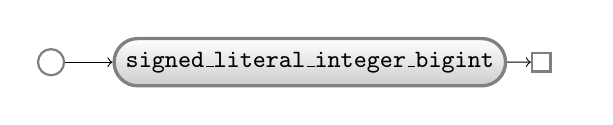
\begin{tikzpicture}
  \matrix[column sep=\ruleMatrixColumnSeparation, row sep=\ruleMatrixRowSeparation] {
    \node (P0start) [firstPoint] {}; & & \node (p0-2) [terminal] {signed\_literal\_integer\_bigint}; & \node (p0-3) [lastPoint] {}; & \\
  };
  \draw[->] (P0start) -- (p0-2) ;
  \draw[->] (p0-2) -- (p0-3) ;
\end{tikzpicture}

\ruleSubsection{gtl\_expression\_parser}{gtl\_expression\_parser}{295}

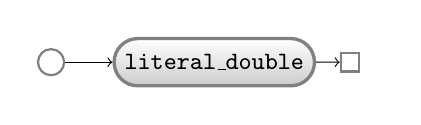
\begin{tikzpicture}
  \matrix[column sep=\ruleMatrixColumnSeparation, row sep=\ruleMatrixRowSeparation] {
    \node (P0start) [firstPoint] {}; & & \node (p0-2) [terminal] {literal\_double}; & \node (p0-3) [lastPoint] {}; & \\
  };
  \draw[->] (P0start) -- (p0-2) ;
  \draw[->] (p0-2) -- (p0-3) ;
\end{tikzpicture}

\ruleSubsection{gtl\_expression\_parser}{gtl\_expression\_parser}{308}

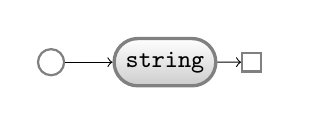
\begin{tikzpicture}
  \matrix[column sep=\ruleMatrixColumnSeparation, row sep=\ruleMatrixRowSeparation] {
    \node (P0start) [firstPoint] {}; & & \node (p0-2) [terminal] {string}; & \node (p0-3) [lastPoint] {}; & \\
  };
  \draw[->] (P0start) -- (p0-2) ;
  \draw[->] (p0-2) -- (p0-3) ;
\end{tikzpicture}

\ruleSubsection{gtl\_expression\_parser}{gtl\_expression\_parser}{321}

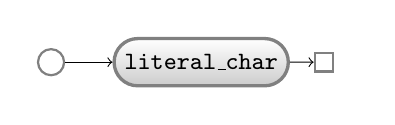
\begin{tikzpicture}
  \matrix[column sep=\ruleMatrixColumnSeparation, row sep=\ruleMatrixRowSeparation] {
    \node (P0start) [firstPoint] {}; & & \node (p0-2) [terminal] {literal\_char}; & \node (p0-3) [lastPoint] {}; & \\
  };
  \draw[->] (P0start) -- (p0-2) ;
  \draw[->] (p0-2) -- (p0-3) ;
\end{tikzpicture}

\ruleSubsection{gtl\_expression\_parser}{gtl\_expression\_parser}{335}

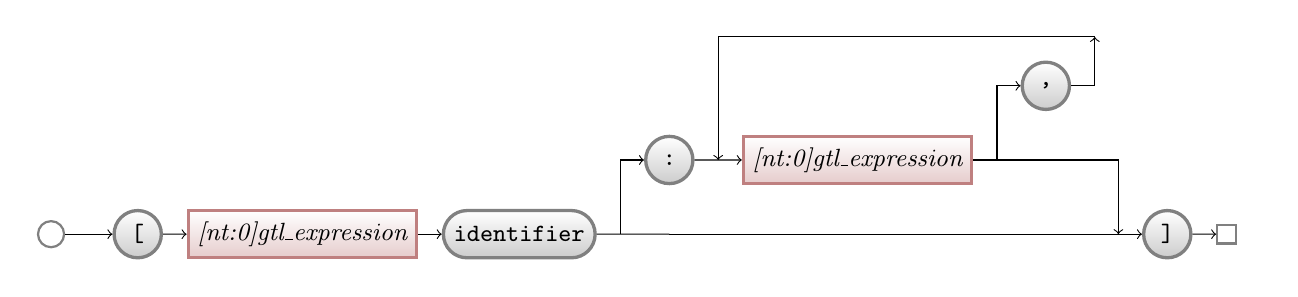
\begin{tikzpicture}
  \matrix[column sep=\ruleMatrixColumnSeparation, row sep=\ruleMatrixRowSeparation] {
    & & & & & & & & & & & \node (p3-11) [point] {}; & \\
    & & & & & & & & & & \node (p2-10) [terminal] {,}; & \\
    & & & & & & \node (p1-6) [terminal] {:}; & \node (p1-7) [point] {}; & \node (p1-8) [nonterminal] {\nonTerminalSymbol{gtl\_expression}{0}}; & \node (p1-9) [point] {}; & \\
    \node (P0start) [firstPoint] {}; & & \node (p0-2) [terminal] {[}; & \node (p0-3) [nonterminal] {\nonTerminalSymbol{gtl\_expression}{0}}; & \node (p0-4) [terminal] {identifier}; & \node (p0-5) [point] {}; & \node (p0-6) [point] {}; & & & & & & \node (p0-12) [point] {}; & \node (p0-13) [terminal] {]}; & \node (p0-14) [lastPoint] {}; & \\
  };
  \draw[->] (P0start) -- (p0-2) ;
  \draw[->] (p0-2) -- (p0-3) ;
  \draw[->] (p0-3) -- (p0-4) ;
  \draw (p0-4) -- (p0-6) ;
  \draw[->] (p0-5) |- (p1-6) ;
  \draw[->] (p1-6) -- (p1-8) ;
  \draw[->] (p1-9) |- (p2-10) ;
  \draw[->] (p3-11) -| (p1-7) ;
  \draw[->] (p2-10) -| (p3-11) ;
  \draw (p0-6) -- (p0-12) ;
  \draw[->] (p1-8) -| (p0-12) ;
  \draw[->] (p0-12) -- (p0-13) ;
  \draw[->] (p0-13) -- (p0-14) ;
\end{tikzpicture}

\ruleSubsection{gtl\_expression\_parser}{gtl\_expression\_parser}{369}

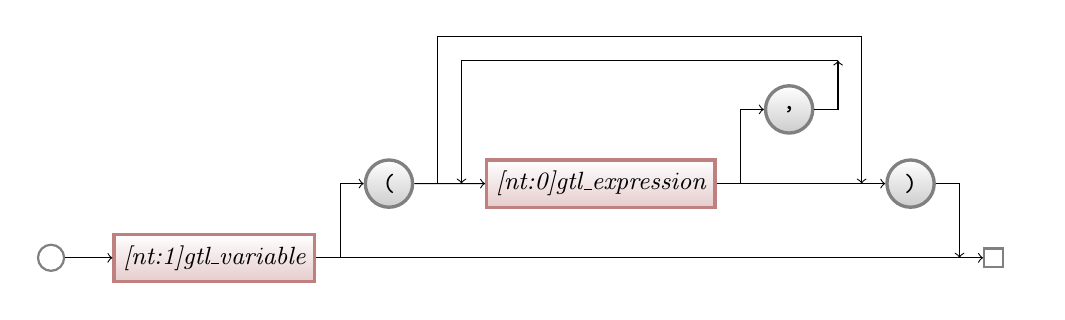
\begin{tikzpicture}
  \matrix[column sep=\ruleMatrixColumnSeparation, row sep=\ruleMatrixRowSeparation] {
    & & & & & & \node (p4-6) [point] {}; & \\
    & & & & & & & & & & \node (p3-10) [point] {}; & \\
    & & & & & & & & & \node (p2-9) [terminal] {,}; & \\
    & & & & \node (p1-4) [terminal] {(}; & \node (p1-5) [point] {}; & \node (p1-6) [point] {}; & \node (p1-7) [nonterminal] {\nonTerminalSymbol{gtl\_expression}{0}}; & \node (p1-8) [point] {}; & & & \node (p1-11) [point] {}; & \node (p1-12) [terminal] {)}; & \\
    \node (P0start) [firstPoint] {}; & & \node (p0-2) [nonterminal] {\nonTerminalSymbol{gtl\_variable}{1}}; & \node (p0-3) [point] {}; & \node (p0-4) [point] {}; & & & & & & & & & \node (p0-13) [point] {}; & \node (p0-14) [lastPoint] {}; & \\
  };
  \draw[->] (P0start) -- (p0-2) ;
  \draw (p0-2) -- (p0-4) ;
  \draw[->] (p0-3) |- (p1-4) ;
  \draw[->] (p1-4) -- (p1-7) ;
  \draw[->] (p1-8) |- (p2-9) ;
  \draw[->] (p3-10) -| (p1-6) ;
  \draw[->] (p2-9) -| (p3-10) ;
  \draw (p1-5) |- (p4-6) ;
  \draw (p1-7) -- (p1-11) ;
  \draw[->] (p4-6) -| (p1-11) ;
  \draw[->] (p1-11) -- (p1-12) ;
  \draw (p0-4) -- (p0-13) ;
  \draw[->] (p1-12) -| (p0-13) ;
  \draw[->] (p0-13) -- (p0-14) ;
\end{tikzpicture}

\ruleSubsection{gtl\_expression\_parser}{gtl\_expression\_parser}{401}

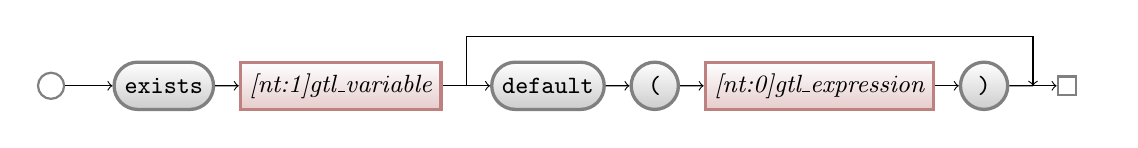
\begin{tikzpicture}
  \matrix[column sep=\ruleMatrixColumnSeparation, row sep=\ruleMatrixRowSeparation] {
    & & & & & \node (p1-5) [point] {}; & \\
    \node (P0start) [firstPoint] {}; & & \node (p0-2) [terminal] {exists}; & \node (p0-3) [nonterminal] {\nonTerminalSymbol{gtl\_variable}{1}}; & \node (p0-4) [point] {}; & \node (p0-5) [terminal] {default}; & \node (p0-6) [terminal] {(}; & \node (p0-7) [nonterminal] {\nonTerminalSymbol{gtl\_expression}{0}}; & \node (p0-8) [terminal] {)}; & \node (p0-9) [point] {}; & \node (p0-10) [lastPoint] {}; & \\
  };
  \draw[->] (P0start) -- (p0-2) ;
  \draw[->] (p0-2) -- (p0-3) ;
  \draw[->] (p0-3) -- (p0-5) ;
  \draw[->] (p0-5) -- (p0-6) ;
  \draw[->] (p0-6) -- (p0-7) ;
  \draw[->] (p0-7) -- (p0-8) ;
  \draw (p0-4) |- (p1-5) ;
  \draw (p0-8) -- (p0-9) ;
  \draw[->] (p1-5) -| (p0-9) ;
  \draw[->] (p0-9) -- (p0-10) ;
\end{tikzpicture}

\ruleSubsection{gtl\_expression\_parser}{gtl\_expression\_parser}{420}

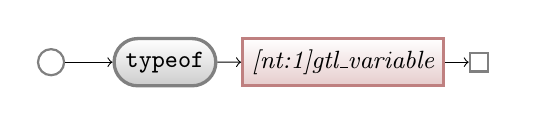
\begin{tikzpicture}
  \matrix[column sep=\ruleMatrixColumnSeparation, row sep=\ruleMatrixRowSeparation] {
    \node (P0start) [firstPoint] {}; & & \node (p0-2) [terminal] {typeof}; & \node (p0-3) [nonterminal] {\nonTerminalSymbol{gtl\_variable}{1}}; & \node (p0-4) [lastPoint] {}; & \\
  };
  \draw[->] (P0start) -- (p0-2) ;
  \draw[->] (p0-2) -- (p0-3) ;
  \draw[->] (p0-3) -- (p0-4) ;
\end{tikzpicture}

\ruleSubsection{gtl\_expression\_parser}{gtl\_expression\_parser}{429}

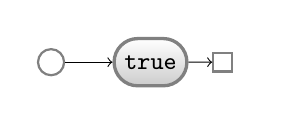
\begin{tikzpicture}
  \matrix[column sep=\ruleMatrixColumnSeparation, row sep=\ruleMatrixRowSeparation] {
    \node (P0start) [firstPoint] {}; & & \node (p0-2) [terminal] {true}; & \node (p0-3) [lastPoint] {}; & \\
  };
  \draw[->] (P0start) -- (p0-2) ;
  \draw[->] (p0-2) -- (p0-3) ;
\end{tikzpicture}

\ruleSubsection{gtl\_expression\_parser}{gtl\_expression\_parser}{445}

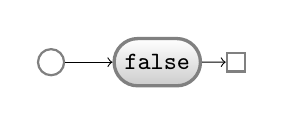
\begin{tikzpicture}
  \matrix[column sep=\ruleMatrixColumnSeparation, row sep=\ruleMatrixRowSeparation] {
    \node (P0start) [firstPoint] {}; & & \node (p0-2) [terminal] {false}; & \node (p0-3) [lastPoint] {}; & \\
  };
  \draw[->] (P0start) -- (p0-2) ;
  \draw[->] (p0-2) -- (p0-3) ;
\end{tikzpicture}

\ruleSubsection{gtl\_expression\_parser}{gtl\_expression\_parser}{461}

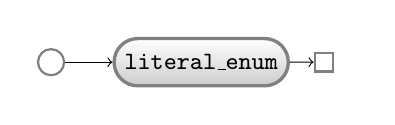
\begin{tikzpicture}
  \matrix[column sep=\ruleMatrixColumnSeparation, row sep=\ruleMatrixRowSeparation] {
    \node (P0start) [firstPoint] {}; & & \node (p0-2) [terminal] {literal\_enum}; & \node (p0-3) [lastPoint] {}; & \\
  };
  \draw[->] (P0start) -- (p0-2) ;
  \draw[->] (p0-2) -- (p0-3) ;
\end{tikzpicture}

\ruleSubsection{gtl\_expression\_parser}{gtl\_expression\_parser}{477}

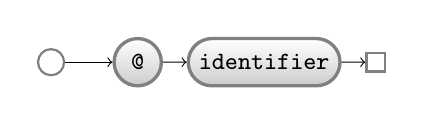
\begin{tikzpicture}
  \matrix[column sep=\ruleMatrixColumnSeparation, row sep=\ruleMatrixRowSeparation] {
    \node (P0start) [firstPoint] {}; & & \node (p0-2) [terminal] {@}; & \node (p0-3) [terminal] {identifier}; & \node (p0-4) [lastPoint] {}; & \\
  };
  \draw[->] (P0start) -- (p0-2) ;
  \draw[->] (p0-2) -- (p0-3) ;
  \draw[->] (p0-3) -- (p0-4) ;
\end{tikzpicture}

\ruleSubsection{gtl\_expression\_parser}{gtl\_expression\_parser}{514}

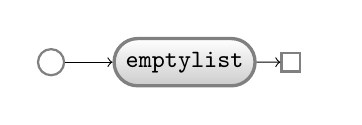
\begin{tikzpicture}
  \matrix[column sep=\ruleMatrixColumnSeparation, row sep=\ruleMatrixRowSeparation] {
    \node (P0start) [firstPoint] {}; & & \node (p0-2) [terminal] {emptylist}; & \node (p0-3) [lastPoint] {}; & \\
  };
  \draw[->] (P0start) -- (p0-2) ;
  \draw[->] (p0-2) -- (p0-3) ;
\end{tikzpicture}

\ruleSubsection{gtl\_expression\_parser}{gtl\_expression\_parser}{533}

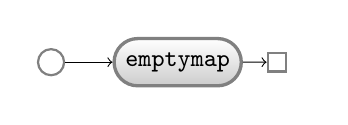
\begin{tikzpicture}
  \matrix[column sep=\ruleMatrixColumnSeparation, row sep=\ruleMatrixRowSeparation] {
    \node (P0start) [firstPoint] {}; & & \node (p0-2) [terminal] {emptymap}; & \node (p0-3) [lastPoint] {}; & \\
  };
  \draw[->] (P0start) -- (p0-2) ;
  \draw[->] (p0-2) -- (p0-3) ;
\end{tikzpicture}

\ruleSubsection{gtl\_expression\_parser}{gtl\_expression\_parser}{552}

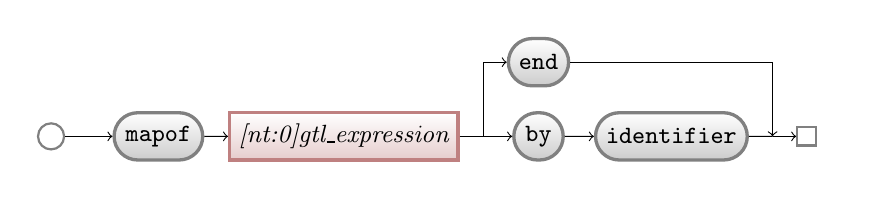
\begin{tikzpicture}
  \matrix[column sep=\ruleMatrixColumnSeparation, row sep=\ruleMatrixRowSeparation] {
    & & & & & \node (p1-5) [terminal] {end}; & \\
    \node (P0start) [firstPoint] {}; & & \node (p0-2) [terminal] {mapof}; & \node (p0-3) [nonterminal] {\nonTerminalSymbol{gtl\_expression}{0}}; & \node (p0-4) [point] {}; & \node (p0-5) [terminal] {by}; & \node (p0-6) [terminal] {identifier}; & \node (p0-7) [point] {}; & \node (p0-8) [lastPoint] {}; & \\
  };
  \draw[->] (P0start) -- (p0-2) ;
  \draw[->] (p0-2) -- (p0-3) ;
  \draw[->] (p0-3) -- (p0-5) ;
  \draw[->] (p0-5) -- (p0-6) ;
  \draw[->] (p0-4) |- (p1-5) ;
  \draw (p0-6) -- (p0-7) ;
  \draw[->] (p1-5) -| (p0-7) ;
  \draw[->] (p0-7) -- (p0-8) ;
\end{tikzpicture}

\ruleSubsection{gtl\_expression\_parser}{gtl\_expression\_parser}{576}

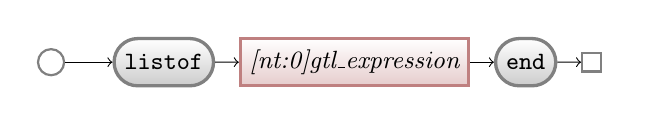
\begin{tikzpicture}
  \matrix[column sep=\ruleMatrixColumnSeparation, row sep=\ruleMatrixRowSeparation] {
    \node (P0start) [firstPoint] {}; & & \node (p0-2) [terminal] {listof}; & \node (p0-3) [nonterminal] {\nonTerminalSymbol{gtl\_expression}{0}}; & \node (p0-4) [terminal] {end}; & \node (p0-5) [lastPoint] {}; & \\
  };
  \draw[->] (P0start) -- (p0-2) ;
  \draw[->] (p0-2) -- (p0-3) ;
  \draw[->] (p0-3) -- (p0-4) ;
  \draw[->] (p0-4) -- (p0-5) ;
\end{tikzpicture}

\ruleSubsection{gtl\_expression\_parser}{gtl\_expression\_parser}{587}

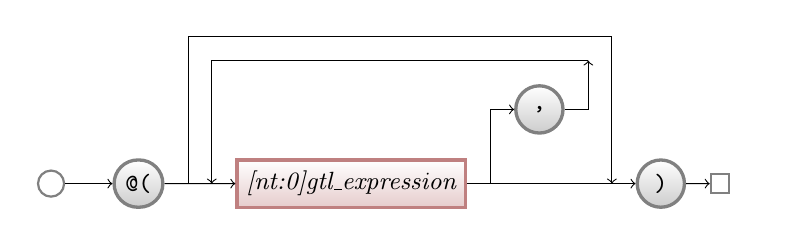
\begin{tikzpicture}
  \matrix[column sep=\ruleMatrixColumnSeparation, row sep=\ruleMatrixRowSeparation] {
    & & & & \node (p3-4) [point] {}; & \\
    & & & & & & & & \node (p2-8) [point] {}; & \\
    & & & & & & & \node (p1-7) [terminal] {,}; & \\
    \node (P0start) [firstPoint] {}; & & \node (p0-2) [terminal] {@(}; & \node (p0-3) [point] {}; & \node (p0-4) [point] {}; & \node (p0-5) [nonterminal] {\nonTerminalSymbol{gtl\_expression}{0}}; & \node (p0-6) [point] {}; & & & \node (p0-9) [point] {}; & \node (p0-10) [terminal] {)}; & \node (p0-11) [lastPoint] {}; & \\
  };
  \draw[->] (P0start) -- (p0-2) ;
  \draw[->] (p0-2) -- (p0-5) ;
  \draw[->] (p0-6) |- (p1-7) ;
  \draw[->] (p2-8) -| (p0-4) ;
  \draw[->] (p1-7) -| (p2-8) ;
  \draw (p0-3) |- (p3-4) ;
  \draw (p0-5) -- (p0-9) ;
  \draw[->] (p3-4) -| (p0-9) ;
  \draw[->] (p0-9) -- (p0-10) ;
  \draw[->] (p0-10) -- (p0-11) ;
\end{tikzpicture}

\ruleSubsection{gtl\_expression\_parser}{gtl\_expression\_parser}{606}

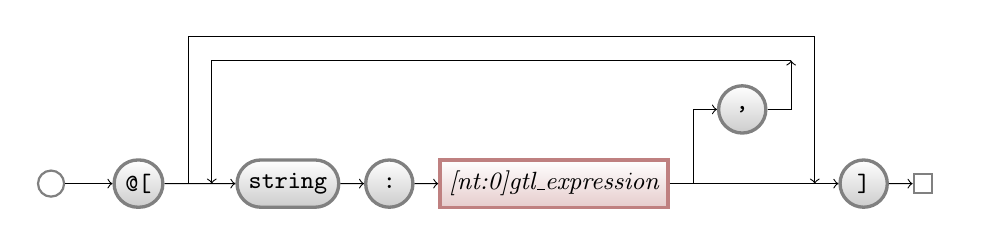
\begin{tikzpicture}
  \matrix[column sep=\ruleMatrixColumnSeparation, row sep=\ruleMatrixRowSeparation] {
    & & & & \node (p3-4) [point] {}; & \\
    & & & & & & & & & & \node (p2-10) [point] {}; & \\
    & & & & & & & & & \node (p1-9) [terminal] {,}; & \\
    \node (P0start) [firstPoint] {}; & & \node (p0-2) [terminal] {@[}; & \node (p0-3) [point] {}; & \node (p0-4) [point] {}; & \node (p0-5) [terminal] {string}; & \node (p0-6) [terminal] {:}; & \node (p0-7) [nonterminal] {\nonTerminalSymbol{gtl\_expression}{0}}; & \node (p0-8) [point] {}; & & & \node (p0-11) [point] {}; & \node (p0-12) [terminal] {]}; & \node (p0-13) [lastPoint] {}; & \\
  };
  \draw[->] (P0start) -- (p0-2) ;
  \draw[->] (p0-2) -- (p0-5) ;
  \draw[->] (p0-5) -- (p0-6) ;
  \draw[->] (p0-6) -- (p0-7) ;
  \draw[->] (p0-8) |- (p1-9) ;
  \draw[->] (p2-10) -| (p0-4) ;
  \draw[->] (p1-9) -| (p2-10) ;
  \draw (p0-3) |- (p3-4) ;
  \draw (p0-7) -- (p0-11) ;
  \draw[->] (p3-4) -| (p0-11) ;
  \draw[->] (p0-11) -- (p0-12) ;
  \draw[->] (p0-12) -- (p0-13) ;
\end{tikzpicture}

\ruleSubsection{gtl\_expression\_parser}{gtl\_expression\_parser}{627}

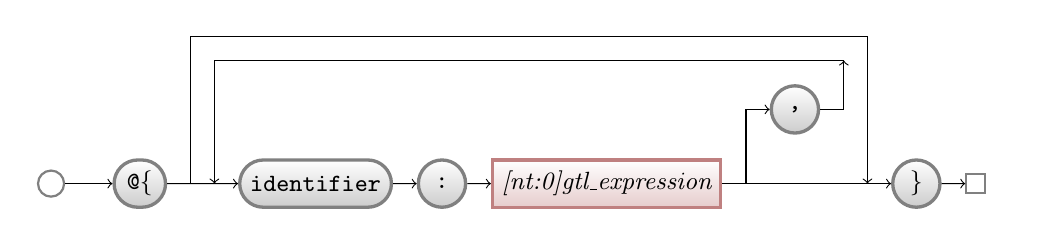
\begin{tikzpicture}
  \matrix[column sep=\ruleMatrixColumnSeparation, row sep=\ruleMatrixRowSeparation] {
    & & & & \node (p3-4) [point] {}; & \\
    & & & & & & & & & & \node (p2-10) [point] {}; & \\
    & & & & & & & & & \node (p1-9) [terminal] {,}; & \\
    \node (P0start) [firstPoint] {}; & & \node (p0-2) [terminal] {@\{}; & \node (p0-3) [point] {}; & \node (p0-4) [point] {}; & \node (p0-5) [terminal] {identifier}; & \node (p0-6) [terminal] {:}; & \node (p0-7) [nonterminal] {\nonTerminalSymbol{gtl\_expression}{0}}; & \node (p0-8) [point] {}; & & & \node (p0-11) [point] {}; & \node (p0-12) [terminal] {\}}; & \node (p0-13) [lastPoint] {}; & \\
  };
  \draw[->] (P0start) -- (p0-2) ;
  \draw[->] (p0-2) -- (p0-5) ;
  \draw[->] (p0-5) -- (p0-6) ;
  \draw[->] (p0-6) -- (p0-7) ;
  \draw[->] (p0-8) |- (p1-9) ;
  \draw[->] (p2-10) -| (p0-4) ;
  \draw[->] (p1-9) -| (p2-10) ;
  \draw (p0-3) |- (p3-4) ;
  \draw (p0-7) -- (p0-11) ;
  \draw[->] (p3-4) -| (p0-11) ;
  \draw[->] (p0-11) -- (p0-12) ;
  \draw[->] (p0-12) -- (p0-13) ;
\end{tikzpicture}

\ruleSubsection{gtl\_expression\_parser}{gtl\_expression\_parser}{648}

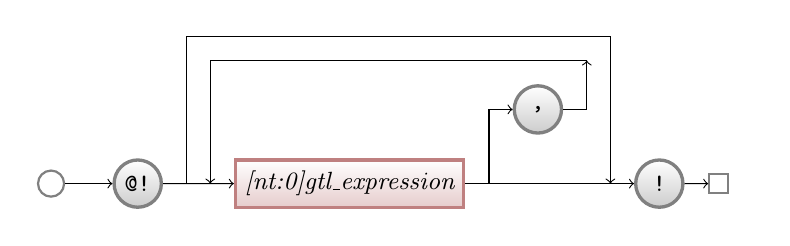
\begin{tikzpicture}
  \matrix[column sep=\ruleMatrixColumnSeparation, row sep=\ruleMatrixRowSeparation] {
    & & & & \node (p3-4) [point] {}; & \\
    & & & & & & & & \node (p2-8) [point] {}; & \\
    & & & & & & & \node (p1-7) [terminal] {,}; & \\
    \node (P0start) [firstPoint] {}; & & \node (p0-2) [terminal] {@!}; & \node (p0-3) [point] {}; & \node (p0-4) [point] {}; & \node (p0-5) [nonterminal] {\nonTerminalSymbol{gtl\_expression}{0}}; & \node (p0-6) [point] {}; & & & \node (p0-9) [point] {}; & \node (p0-10) [terminal] {!}; & \node (p0-11) [lastPoint] {}; & \\
  };
  \draw[->] (P0start) -- (p0-2) ;
  \draw[->] (p0-2) -- (p0-5) ;
  \draw[->] (p0-6) |- (p1-7) ;
  \draw[->] (p2-8) -| (p0-4) ;
  \draw[->] (p1-7) -| (p2-8) ;
  \draw (p0-3) |- (p3-4) ;
  \draw (p0-5) -- (p0-9) ;
  \draw[->] (p3-4) -| (p0-9) ;
  \draw[->] (p0-9) -- (p0-10) ;
  \draw[->] (p0-10) -- (p0-11) ;
\end{tikzpicture}

\ruleSubsection{gtl\_expression\_parser}{gtl\_expression\_parser}{667}

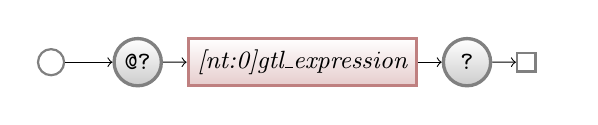
\begin{tikzpicture}
  \matrix[column sep=\ruleMatrixColumnSeparation, row sep=\ruleMatrixRowSeparation] {
    \node (P0start) [firstPoint] {}; & & \node (p0-2) [terminal] {@?}; & \node (p0-3) [nonterminal] {\nonTerminalSymbol{gtl\_expression}{0}}; & \node (p0-4) [terminal] {?}; & \node (p0-5) [lastPoint] {}; & \\
  };
  \draw[->] (P0start) -- (p0-2) ;
  \draw[->] (p0-2) -- (p0-3) ;
  \draw[->] (p0-3) -- (p0-4) ;
  \draw[->] (p0-4) -- (p0-5) ;
\end{tikzpicture}

\ruleSubsection{gtl\_expression\_parser}{gtl\_expression\_parser}{678}

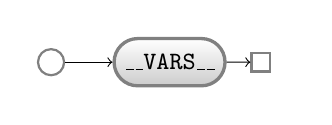
\begin{tikzpicture}
  \matrix[column sep=\ruleMatrixColumnSeparation, row sep=\ruleMatrixRowSeparation] {
    \node (P0start) [firstPoint] {}; & & \node (p0-2) [terminal] {\_\_VARS\_\_}; & \node (p0-3) [lastPoint] {}; & \\
  };
  \draw[->] (P0start) -- (p0-2) ;
  \draw[->] (p0-2) -- (p0-3) ;
\end{tikzpicture}

\nonTerminalSection{gtl\_file\_name}{9}

\ruleSubsection{gtl\_parser}{gtl\_parser}{443}

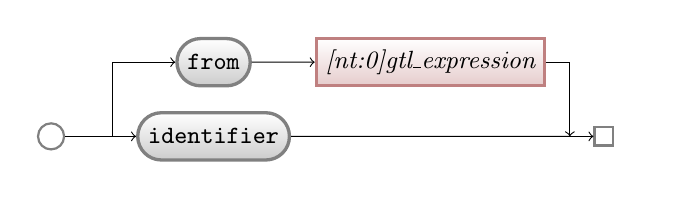
\begin{tikzpicture}
  \matrix[column sep=\ruleMatrixColumnSeparation, row sep=\ruleMatrixRowSeparation] {
    & & & \node (p1-3) [terminal] {from}; & \node (p1-4) [nonterminal] {\nonTerminalSymbol{gtl\_expression}{0}}; & \\
    \node (P0start) [firstPoint] {}; & & \node (p0-2) [point] {}; & \node (p0-3) [terminal] {identifier}; & & \node (p0-5) [point] {}; & \node (p0-6) [lastPoint] {}; & \\
  };
  \draw[->] (P0start) -- (p0-3) ;
  \draw[->] (p0-2) |- (p1-3) ;
  \draw[->] (p1-3) -- (p1-4) ;
  \draw (p0-3) -- (p0-5) ;
  \draw[->] (p1-4) -| (p0-5) ;
  \draw[->] (p0-5) -- (p0-6) ;
\end{tikzpicture}

\nonTerminalSection{gtl\_import}{3}

\ruleSubsection{gtl\_instruction\_parser}{gtl\_instruction\_parser}{391}

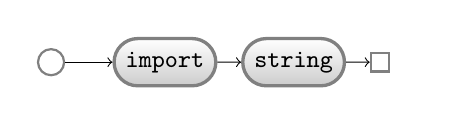
\begin{tikzpicture}
  \matrix[column sep=\ruleMatrixColumnSeparation, row sep=\ruleMatrixRowSeparation] {
    \node (P0start) [firstPoint] {}; & & \node (p0-2) [terminal] {import}; & \node (p0-3) [terminal] {string}; & \node (p0-4) [lastPoint] {}; & \\
  };
  \draw[->] (P0start) -- (p0-2) ;
  \draw[->] (p0-2) -- (p0-3) ;
  \draw[->] (p0-3) -- (p0-4) ;
\end{tikzpicture}

\nonTerminalSection{gtl\_relation\_factor}{11}

\ruleSubsection{gtl\_expression\_parser}{gtl\_expression\_parser}{69}

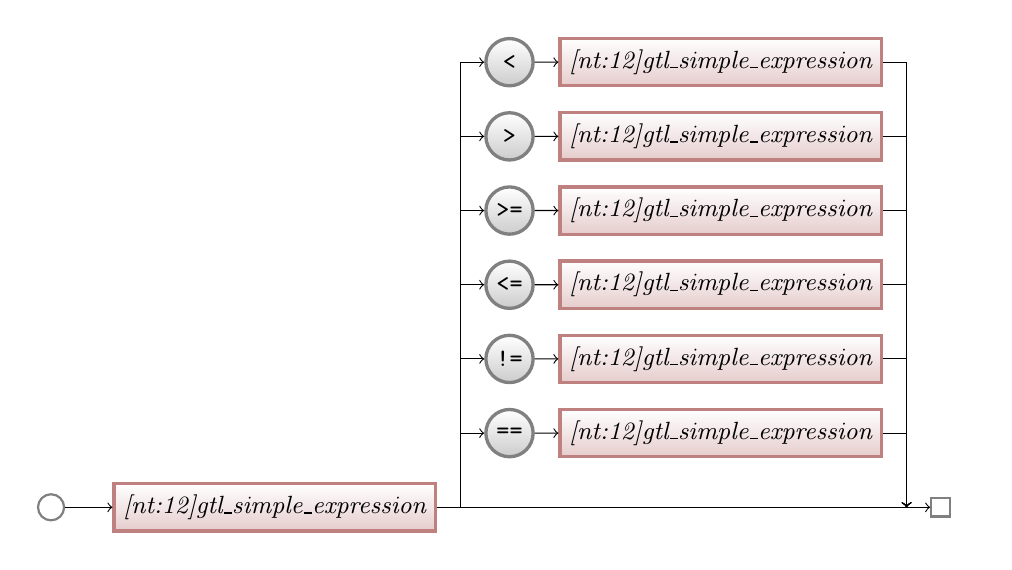
\begin{tikzpicture}
  \matrix[column sep=\ruleMatrixColumnSeparation, row sep=\ruleMatrixRowSeparation] {
    & & & & \node (p6-4) [terminal] {<}; & \node (p6-5) [nonterminal] {\nonTerminalSymbol{gtl\_simple\_expression}{12}}; & \\
    & & & & \node (p5-4) [terminal] {>}; & \node (p5-5) [nonterminal] {\nonTerminalSymbol{gtl\_simple\_expression}{12}}; & \\
    & & & & \node (p4-4) [terminal] {>=}; & \node (p4-5) [nonterminal] {\nonTerminalSymbol{gtl\_simple\_expression}{12}}; & \\
    & & & & \node (p3-4) [terminal] {<=}; & \node (p3-5) [nonterminal] {\nonTerminalSymbol{gtl\_simple\_expression}{12}}; & \\
    & & & & \node (p2-4) [terminal] {!=}; & \node (p2-5) [nonterminal] {\nonTerminalSymbol{gtl\_simple\_expression}{12}}; & \\
    & & & & \node (p1-4) [terminal] {==}; & \node (p1-5) [nonterminal] {\nonTerminalSymbol{gtl\_simple\_expression}{12}}; & \\
    \node (P0start) [firstPoint] {}; & & \node (p0-2) [nonterminal] {\nonTerminalSymbol{gtl\_simple\_expression}{12}}; & \node (p0-3) [point] {}; & \node (p0-4) [point] {}; & & \node (p0-6) [point] {}; & \node (p0-7) [lastPoint] {}; & \\
  };
  \draw[->] (P0start) -- (p0-2) ;
  \draw (p0-2) -- (p0-4) ;
  \draw[->] (p0-3) |- (p1-4) ;
  \draw[->] (p1-4) -- (p1-5) ;
  \draw[->] (p0-3) |- (p2-4) ;
  \draw[->] (p2-4) -- (p2-5) ;
  \draw[->] (p0-3) |- (p3-4) ;
  \draw[->] (p3-4) -- (p3-5) ;
  \draw[->] (p0-3) |- (p4-4) ;
  \draw[->] (p4-4) -- (p4-5) ;
  \draw[->] (p0-3) |- (p5-4) ;
  \draw[->] (p5-4) -- (p5-5) ;
  \draw[->] (p0-3) |- (p6-4) ;
  \draw[->] (p6-4) -- (p6-5) ;
  \draw (p0-4) -- (p0-6) ;
  \draw[->] (p1-5) -| (p0-6) ;
  \draw[->] (p2-5) -| (p0-6) ;
  \draw[->] (p3-5) -| (p0-6) ;
  \draw[->] (p4-5) -| (p0-6) ;
  \draw[->] (p5-5) -| (p0-6) ;
  \draw[->] (p6-5) -| (p0-6) ;
  \draw[->] (p0-6) -- (p0-7) ;
\end{tikzpicture}

\nonTerminalSection{gtl\_relation\_term}{10}

\ruleSubsection{gtl\_expression\_parser}{gtl\_expression\_parser}{53}

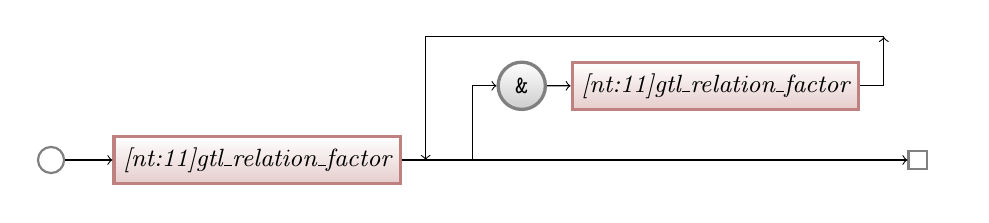
\begin{tikzpicture}
  \matrix[column sep=\ruleMatrixColumnSeparation, row sep=\ruleMatrixRowSeparation] {
    & & & & & & & & \node (p2-8) [point] {}; & \\
    & & & & & & \node (p1-6) [terminal] {\&}; & \node (p1-7) [nonterminal] {\nonTerminalSymbol{gtl\_relation\_factor}{11}}; & \\
    \node (P0start) [firstPoint] {}; & & \node (p0-2) [nonterminal] {\nonTerminalSymbol{gtl\_relation\_factor}{11}}; & \node (p0-3) [point] {}; & \node (p0-4) [point] {}; & \node (p0-5) [point] {}; & & & & \node (p0-9) [lastPoint] {}; & \\
  };
  \draw[->] (P0start) -- (p0-2) ;
  \draw (p0-2) -- (p0-4) ;
  \draw[->] (p0-5) |- (p1-6) ;
  \draw[->] (p1-6) -- (p1-7) ;
  \draw[->] (p2-8) -| (p0-3) ;
  \draw[->] (p1-7) -| (p2-8) ;
  \draw[->] (p0-4) -- (p0-9) ;
\end{tikzpicture}

\nonTerminalSection{gtl\_simple\_expression}{12}

\ruleSubsection{gtl\_expression\_parser}{gtl\_expression\_parser}{117}

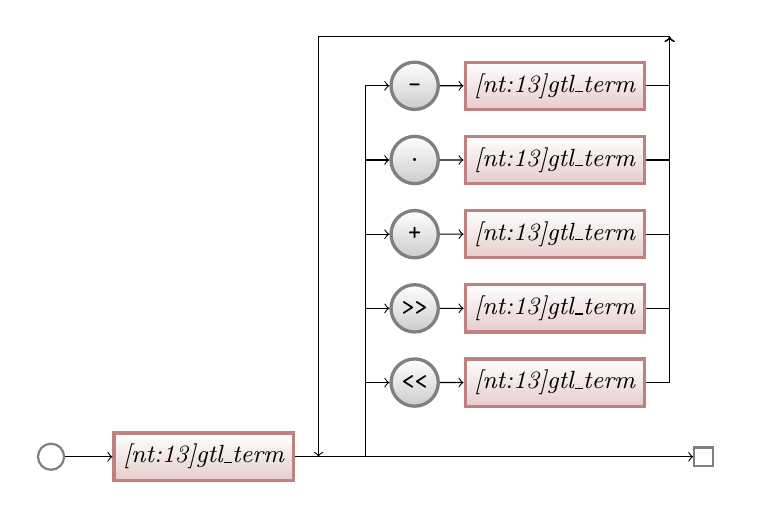
\begin{tikzpicture}
  \matrix[column sep=\ruleMatrixColumnSeparation, row sep=\ruleMatrixRowSeparation] {
    & & & & & & & & \node (p6-8) [point] {}; & \\
    & & & & & & \node (p5-6) [terminal] {-}; & \node (p5-7) [nonterminal] {\nonTerminalSymbol{gtl\_term}{13}}; & \\
    & & & & & & \node (p4-6) [terminal] {.}; & \node (p4-7) [nonterminal] {\nonTerminalSymbol{gtl\_term}{13}}; & \\
    & & & & & & \node (p3-6) [terminal] {+}; & \node (p3-7) [nonterminal] {\nonTerminalSymbol{gtl\_term}{13}}; & \\
    & & & & & & \node (p2-6) [terminal] {>>}; & \node (p2-7) [nonterminal] {\nonTerminalSymbol{gtl\_term}{13}}; & \\
    & & & & & & \node (p1-6) [terminal] {<<}; & \node (p1-7) [nonterminal] {\nonTerminalSymbol{gtl\_term}{13}}; & \\
    \node (P0start) [firstPoint] {}; & & \node (p0-2) [nonterminal] {\nonTerminalSymbol{gtl\_term}{13}}; & \node (p0-3) [point] {}; & \node (p0-4) [point] {}; & \node (p0-5) [point] {}; & & & & \node (p0-9) [lastPoint] {}; & \\
  };
  \draw[->] (P0start) -- (p0-2) ;
  \draw (p0-2) -- (p0-4) ;
  \draw[->] (p0-5) |- (p1-6) ;
  \draw[->] (p1-6) -- (p1-7) ;
  \draw[->] (p0-5) |- (p2-6) ;
  \draw[->] (p2-6) -- (p2-7) ;
  \draw[->] (p0-5) |- (p3-6) ;
  \draw[->] (p3-6) -- (p3-7) ;
  \draw[->] (p0-5) |- (p4-6) ;
  \draw[->] (p4-6) -- (p4-7) ;
  \draw[->] (p0-5) |- (p5-6) ;
  \draw[->] (p5-6) -- (p5-7) ;
  \draw[->] (p6-8) -| (p0-3) ;
  \draw[->] (p1-7) -| (p6-8) ;
  \draw[->] (p2-7) -| (p6-8) ;
  \draw[->] (p3-7) -| (p6-8) ;
  \draw[->] (p4-7) -| (p6-8) ;
  \draw[->] (p5-7) -| (p6-8) ;
  \draw[->] (p0-4) -- (p0-9) ;
\end{tikzpicture}

\nonTerminalSection{gtl\_simple\_instruction}{4}

\ruleSubsection{gtl\_instruction\_parser}{gtl\_instruction\_parser}{40}

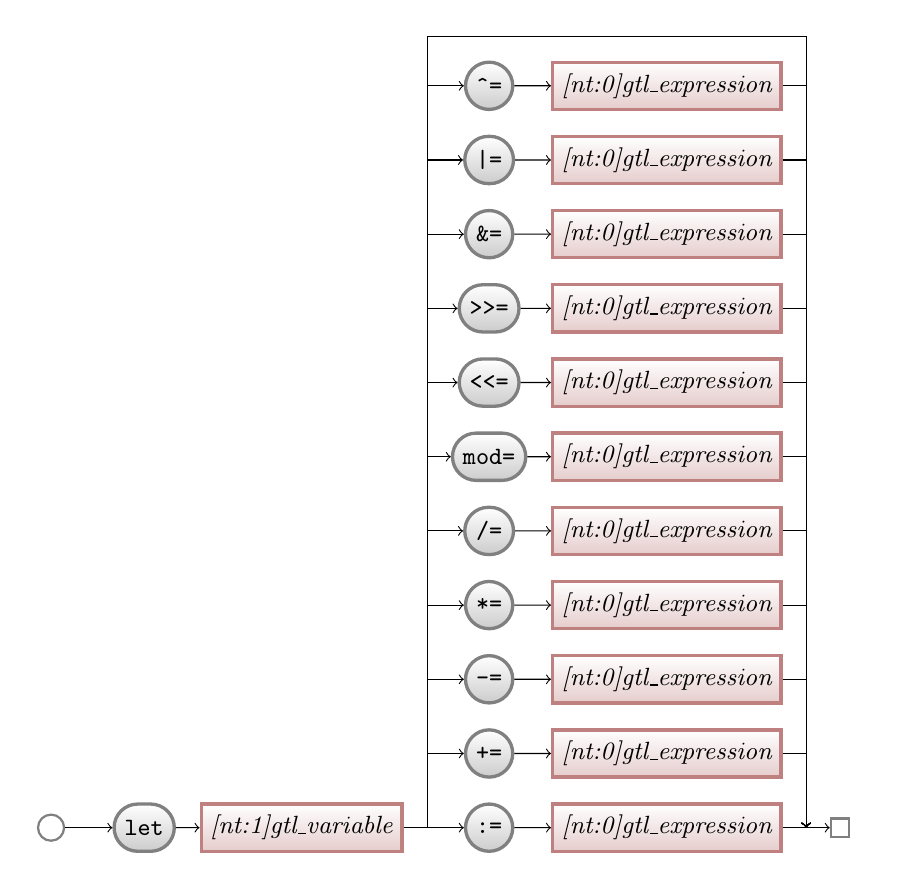
\begin{tikzpicture}
  \matrix[column sep=\ruleMatrixColumnSeparation, row sep=\ruleMatrixRowSeparation] {
    & & & & & \node (p11-5) [point] {}; & \\
    & & & & & \node (p10-5) [terminal] {\verb=^==}; & \node (p10-6) [nonterminal] {\nonTerminalSymbol{gtl\_expression}{0}}; & \\
    & & & & & \node (p9-5) [terminal] {|=}; & \node (p9-6) [nonterminal] {\nonTerminalSymbol{gtl\_expression}{0}}; & \\
    & & & & & \node (p8-5) [terminal] {\&=}; & \node (p8-6) [nonterminal] {\nonTerminalSymbol{gtl\_expression}{0}}; & \\
    & & & & & \node (p7-5) [terminal] {>>=}; & \node (p7-6) [nonterminal] {\nonTerminalSymbol{gtl\_expression}{0}}; & \\
    & & & & & \node (p6-5) [terminal] {<<=}; & \node (p6-6) [nonterminal] {\nonTerminalSymbol{gtl\_expression}{0}}; & \\
    & & & & & \node (p5-5) [terminal] {mod=}; & \node (p5-6) [nonterminal] {\nonTerminalSymbol{gtl\_expression}{0}}; & \\
    & & & & & \node (p4-5) [terminal] {/=}; & \node (p4-6) [nonterminal] {\nonTerminalSymbol{gtl\_expression}{0}}; & \\
    & & & & & \node (p3-5) [terminal] {*=}; & \node (p3-6) [nonterminal] {\nonTerminalSymbol{gtl\_expression}{0}}; & \\
    & & & & & \node (p2-5) [terminal] {-=}; & \node (p2-6) [nonterminal] {\nonTerminalSymbol{gtl\_expression}{0}}; & \\
    & & & & & \node (p1-5) [terminal] {+=}; & \node (p1-6) [nonterminal] {\nonTerminalSymbol{gtl\_expression}{0}}; & \\
    \node (P0start) [firstPoint] {}; & & \node (p0-2) [terminal] {let}; & \node (p0-3) [nonterminal] {\nonTerminalSymbol{gtl\_variable}{1}}; & \node (p0-4) [point] {}; & \node (p0-5) [terminal] {:=}; & \node (p0-6) [nonterminal] {\nonTerminalSymbol{gtl\_expression}{0}}; & \node (p0-7) [point] {}; & \node (p0-8) [lastPoint] {}; & \\
  };
  \draw[->] (P0start) -- (p0-2) ;
  \draw[->] (p0-2) -- (p0-3) ;
  \draw[->] (p0-3) -- (p0-5) ;
  \draw[->] (p0-5) -- (p0-6) ;
  \draw[->] (p0-4) |- (p1-5) ;
  \draw[->] (p1-5) -- (p1-6) ;
  \draw[->] (p0-4) |- (p2-5) ;
  \draw[->] (p2-5) -- (p2-6) ;
  \draw[->] (p0-4) |- (p3-5) ;
  \draw[->] (p3-5) -- (p3-6) ;
  \draw[->] (p0-4) |- (p4-5) ;
  \draw[->] (p4-5) -- (p4-6) ;
  \draw[->] (p0-4) |- (p5-5) ;
  \draw[->] (p5-5) -- (p5-6) ;
  \draw[->] (p0-4) |- (p6-5) ;
  \draw[->] (p6-5) -- (p6-6) ;
  \draw[->] (p0-4) |- (p7-5) ;
  \draw[->] (p7-5) -- (p7-6) ;
  \draw[->] (p0-4) |- (p8-5) ;
  \draw[->] (p8-5) -- (p8-6) ;
  \draw[->] (p0-4) |- (p9-5) ;
  \draw[->] (p9-5) -- (p9-6) ;
  \draw[->] (p0-4) |- (p10-5) ;
  \draw[->] (p10-5) -- (p10-6) ;
  \draw (p0-4) |- (p11-5) ;
  \draw (p0-6) -- (p0-7) ;
  \draw[->] (p1-6) -| (p0-7) ;
  \draw[->] (p2-6) -| (p0-7) ;
  \draw[->] (p3-6) -| (p0-7) ;
  \draw[->] (p4-6) -| (p0-7) ;
  \draw[->] (p5-6) -| (p0-7) ;
  \draw[->] (p6-6) -| (p0-7) ;
  \draw[->] (p7-6) -| (p0-7) ;
  \draw[->] (p8-6) -| (p0-7) ;
  \draw[->] (p9-6) -| (p0-7) ;
  \draw[->] (p10-6) -| (p0-7) ;
  \draw[->] (p11-5) -| (p0-7) ;
  \draw[->] (p0-7) -- (p0-8) ;
\end{tikzpicture}

\ruleSubsection{gtl\_instruction\_parser}{gtl\_instruction\_parser}{154}

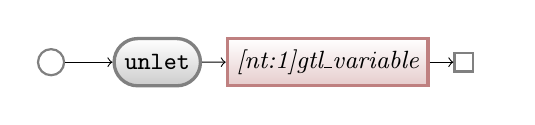
\begin{tikzpicture}
  \matrix[column sep=\ruleMatrixColumnSeparation, row sep=\ruleMatrixRowSeparation] {
    \node (P0start) [firstPoint] {}; & & \node (p0-2) [terminal] {unlet}; & \node (p0-3) [nonterminal] {\nonTerminalSymbol{gtl\_variable}{1}}; & \node (p0-4) [lastPoint] {}; & \\
  };
  \draw[->] (P0start) -- (p0-2) ;
  \draw[->] (p0-2) -- (p0-3) ;
  \draw[->] (p0-3) -- (p0-4) ;
\end{tikzpicture}

\ruleSubsection{gtl\_instruction\_parser}{gtl\_instruction\_parser}{167}

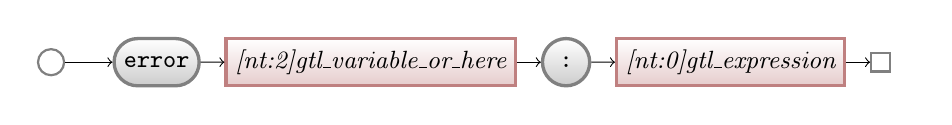
\begin{tikzpicture}
  \matrix[column sep=\ruleMatrixColumnSeparation, row sep=\ruleMatrixRowSeparation] {
    \node (P0start) [firstPoint] {}; & & \node (p0-2) [terminal] {error}; & \node (p0-3) [nonterminal] {\nonTerminalSymbol{gtl\_variable\_or\_here}{2}}; & \node (p0-4) [terminal] {:}; & \node (p0-5) [nonterminal] {\nonTerminalSymbol{gtl\_expression}{0}}; & \node (p0-6) [lastPoint] {}; & \\
  };
  \draw[->] (P0start) -- (p0-2) ;
  \draw[->] (p0-2) -- (p0-3) ;
  \draw[->] (p0-3) -- (p0-4) ;
  \draw[->] (p0-4) -- (p0-5) ;
  \draw[->] (p0-5) -- (p0-6) ;
\end{tikzpicture}

\ruleSubsection{gtl\_instruction\_parser}{gtl\_instruction\_parser}{185}

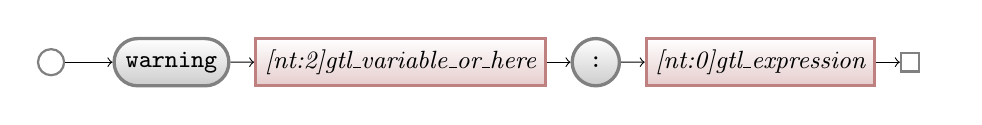
\begin{tikzpicture}
  \matrix[column sep=\ruleMatrixColumnSeparation, row sep=\ruleMatrixRowSeparation] {
    \node (P0start) [firstPoint] {}; & & \node (p0-2) [terminal] {warning}; & \node (p0-3) [nonterminal] {\nonTerminalSymbol{gtl\_variable\_or\_here}{2}}; & \node (p0-4) [terminal] {:}; & \node (p0-5) [nonterminal] {\nonTerminalSymbol{gtl\_expression}{0}}; & \node (p0-6) [lastPoint] {}; & \\
  };
  \draw[->] (P0start) -- (p0-2) ;
  \draw[->] (p0-2) -- (p0-3) ;
  \draw[->] (p0-3) -- (p0-4) ;
  \draw[->] (p0-4) -- (p0-5) ;
  \draw[->] (p0-5) -- (p0-6) ;
\end{tikzpicture}

\ruleSubsection{gtl\_instruction\_parser}{gtl\_instruction\_parser}{203}

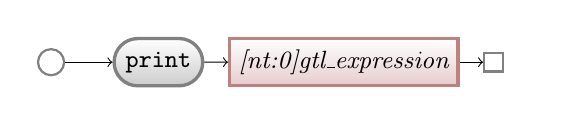
\begin{tikzpicture}
  \matrix[column sep=\ruleMatrixColumnSeparation, row sep=\ruleMatrixRowSeparation] {
    \node (P0start) [firstPoint] {}; & & \node (p0-2) [terminal] {print}; & \node (p0-3) [nonterminal] {\nonTerminalSymbol{gtl\_expression}{0}}; & \node (p0-4) [lastPoint] {}; & \\
  };
  \draw[->] (P0start) -- (p0-2) ;
  \draw[->] (p0-2) -- (p0-3) ;
  \draw[->] (p0-3) -- (p0-4) ;
\end{tikzpicture}

\ruleSubsection{gtl\_instruction\_parser}{gtl\_instruction\_parser}{218}

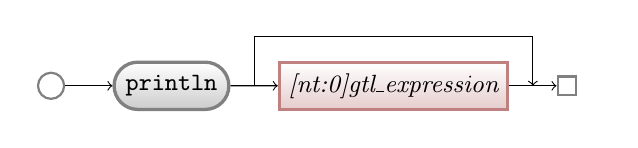
\begin{tikzpicture}
  \matrix[column sep=\ruleMatrixColumnSeparation, row sep=\ruleMatrixRowSeparation] {
    & & & & \node (p1-4) [point] {}; & \\
    \node (P0start) [firstPoint] {}; & & \node (p0-2) [terminal] {println}; & \node (p0-3) [point] {}; & \node (p0-4) [nonterminal] {\nonTerminalSymbol{gtl\_expression}{0}}; & \node (p0-5) [point] {}; & \node (p0-6) [lastPoint] {}; & \\
  };
  \draw[->] (P0start) -- (p0-2) ;
  \draw[->] (p0-2) -- (p0-4) ;
  \draw (p0-3) |- (p1-4) ;
  \draw (p0-4) -- (p0-5) ;
  \draw[->] (p1-4) -| (p0-5) ;
  \draw[->] (p0-5) -- (p0-6) ;
\end{tikzpicture}

\ruleSubsection{gtl\_instruction\_parser}{gtl\_instruction\_parser}{241}

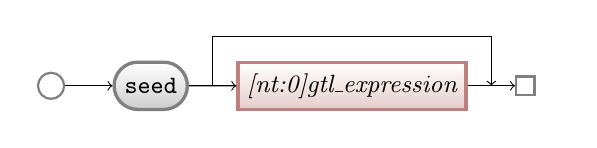
\begin{tikzpicture}
  \matrix[column sep=\ruleMatrixColumnSeparation, row sep=\ruleMatrixRowSeparation] {
    & & & & \node (p1-4) [point] {}; & \\
    \node (P0start) [firstPoint] {}; & & \node (p0-2) [terminal] {seed}; & \node (p0-3) [point] {}; & \node (p0-4) [nonterminal] {\nonTerminalSymbol{gtl\_expression}{0}}; & \node (p0-5) [point] {}; & \node (p0-6) [lastPoint] {}; & \\
  };
  \draw[->] (P0start) -- (p0-2) ;
  \draw[->] (p0-2) -- (p0-4) ;
  \draw (p0-3) |- (p1-4) ;
  \draw (p0-4) -- (p0-5) ;
  \draw[->] (p1-4) -| (p0-5) ;
  \draw[->] (p0-5) -- (p0-6) ;
\end{tikzpicture}

\ruleSubsection{gtl\_instruction\_parser}{gtl\_instruction\_parser}{264}

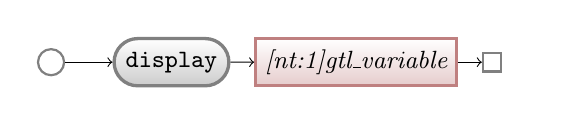
\begin{tikzpicture}
  \matrix[column sep=\ruleMatrixColumnSeparation, row sep=\ruleMatrixRowSeparation] {
    \node (P0start) [firstPoint] {}; & & \node (p0-2) [terminal] {display}; & \node (p0-3) [nonterminal] {\nonTerminalSymbol{gtl\_variable}{1}}; & \node (p0-4) [lastPoint] {}; & \\
  };
  \draw[->] (P0start) -- (p0-2) ;
  \draw[->] (p0-2) -- (p0-3) ;
  \draw[->] (p0-3) -- (p0-4) ;
\end{tikzpicture}

\ruleSubsection{gtl\_instruction\_parser}{gtl\_instruction\_parser}{279}

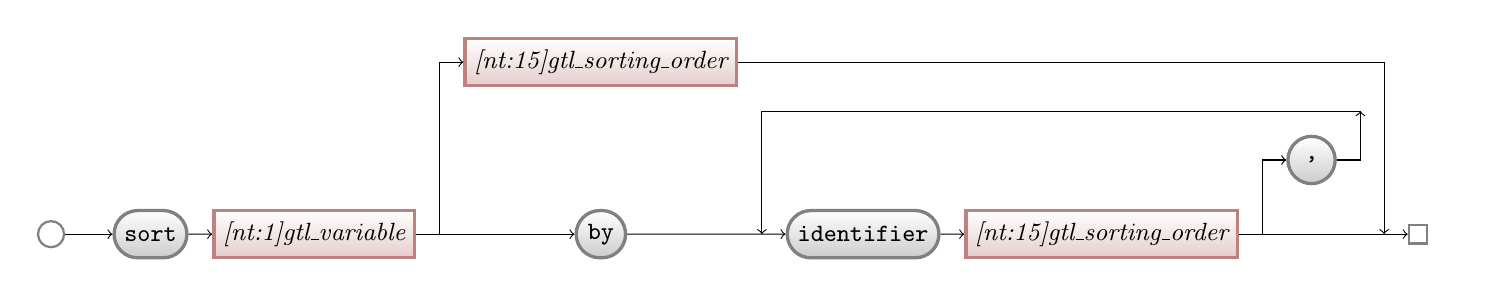
\begin{tikzpicture}
  \matrix[column sep=\ruleMatrixColumnSeparation, row sep=\ruleMatrixRowSeparation] {
    & & & & & \node (p3-5) [nonterminal] {\nonTerminalSymbol{gtl\_sorting\_order}{15}}; & \\
    & & & & & & & & & & & \node (p2-11) [point] {}; & \\
    & & & & & & & & & & \node (p1-10) [terminal] {,}; & \\
    \node (P0start) [firstPoint] {}; & & \node (p0-2) [terminal] {sort}; & \node (p0-3) [nonterminal] {\nonTerminalSymbol{gtl\_variable}{1}}; & \node (p0-4) [point] {}; & \node (p0-5) [terminal] {by}; & \node (p0-6) [point] {}; & \node (p0-7) [terminal] {identifier}; & \node (p0-8) [nonterminal] {\nonTerminalSymbol{gtl\_sorting\_order}{15}}; & \node (p0-9) [point] {}; & & & \node (p0-12) [point] {}; & \node (p0-13) [lastPoint] {}; & \\
  };
  \draw[->] (P0start) -- (p0-2) ;
  \draw[->] (p0-2) -- (p0-3) ;
  \draw[->] (p0-3) -- (p0-5) ;
  \draw[->] (p0-5) -- (p0-7) ;
  \draw[->] (p0-7) -- (p0-8) ;
  \draw[->] (p0-9) |- (p1-10) ;
  \draw[->] (p2-11) -| (p0-6) ;
  \draw[->] (p1-10) -| (p2-11) ;
  \draw[->] (p0-4) |- (p3-5) ;
  \draw (p0-8) -- (p0-12) ;
  \draw[->] (p3-5) -| (p0-12) ;
  \draw[->] (p0-12) -- (p0-13) ;
\end{tikzpicture}

\ruleSubsection{gtl\_instruction\_parser}{gtl\_instruction\_parser}{312}

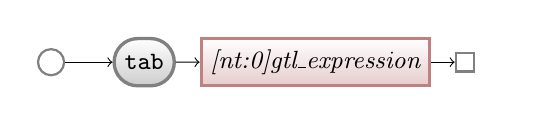
\begin{tikzpicture}
  \matrix[column sep=\ruleMatrixColumnSeparation, row sep=\ruleMatrixRowSeparation] {
    \node (P0start) [firstPoint] {}; & & \node (p0-2) [terminal] {tab}; & \node (p0-3) [nonterminal] {\nonTerminalSymbol{gtl\_expression}{0}}; & \node (p0-4) [lastPoint] {}; & \\
  };
  \draw[->] (P0start) -- (p0-2) ;
  \draw[->] (p0-2) -- (p0-3) ;
  \draw[->] (p0-3) -- (p0-4) ;
\end{tikzpicture}

\ruleSubsection{gtl\_instruction\_parser}{gtl\_instruction\_parser}{326}

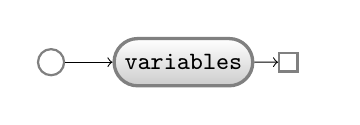
\begin{tikzpicture}
  \matrix[column sep=\ruleMatrixColumnSeparation, row sep=\ruleMatrixRowSeparation] {
    \node (P0start) [firstPoint] {}; & & \node (p0-2) [terminal] {variables}; & \node (p0-3) [lastPoint] {}; & \\
  };
  \draw[->] (P0start) -- (p0-2) ;
  \draw[->] (p0-2) -- (p0-3) ;
\end{tikzpicture}

\ruleSubsection{gtl\_instruction\_parser}{gtl\_instruction\_parser}{338}

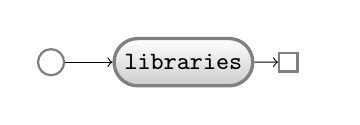
\begin{tikzpicture}
  \matrix[column sep=\ruleMatrixColumnSeparation, row sep=\ruleMatrixRowSeparation] {
    \node (P0start) [firstPoint] {}; & & \node (p0-2) [terminal] {libraries}; & \node (p0-3) [lastPoint] {}; & \\
  };
  \draw[->] (P0start) -- (p0-2) ;
  \draw[->] (p0-2) -- (p0-3) ;
\end{tikzpicture}

\ruleSubsection{gtl\_instruction\_parser}{gtl\_instruction\_parser}{349}

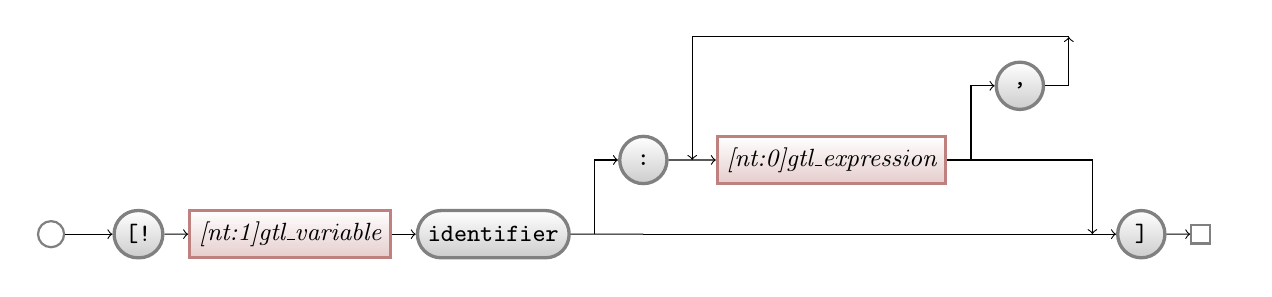
\begin{tikzpicture}
  \matrix[column sep=\ruleMatrixColumnSeparation, row sep=\ruleMatrixRowSeparation] {
    & & & & & & & & & & & \node (p3-11) [point] {}; & \\
    & & & & & & & & & & \node (p2-10) [terminal] {,}; & \\
    & & & & & & \node (p1-6) [terminal] {:}; & \node (p1-7) [point] {}; & \node (p1-8) [nonterminal] {\nonTerminalSymbol{gtl\_expression}{0}}; & \node (p1-9) [point] {}; & \\
    \node (P0start) [firstPoint] {}; & & \node (p0-2) [terminal] {[!}; & \node (p0-3) [nonterminal] {\nonTerminalSymbol{gtl\_variable}{1}}; & \node (p0-4) [terminal] {identifier}; & \node (p0-5) [point] {}; & \node (p0-6) [point] {}; & & & & & & \node (p0-12) [point] {}; & \node (p0-13) [terminal] {]}; & \node (p0-14) [lastPoint] {}; & \\
  };
  \draw[->] (P0start) -- (p0-2) ;
  \draw[->] (p0-2) -- (p0-3) ;
  \draw[->] (p0-3) -- (p0-4) ;
  \draw (p0-4) -- (p0-6) ;
  \draw[->] (p0-5) |- (p1-6) ;
  \draw[->] (p1-6) -- (p1-8) ;
  \draw[->] (p1-9) |- (p2-10) ;
  \draw[->] (p3-11) -| (p1-7) ;
  \draw[->] (p2-10) -| (p3-11) ;
  \draw (p0-6) -- (p0-12) ;
  \draw[->] (p1-8) -| (p0-12) ;
  \draw[->] (p0-12) -- (p0-13) ;
  \draw[->] (p0-13) -- (p0-14) ;
\end{tikzpicture}

\nonTerminalSection{gtl\_sorting\_order}{15}

\ruleSubsection{gtl\_instruction\_parser}{gtl\_instruction\_parser}{378}

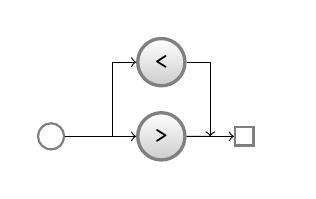
\begin{tikzpicture}
  \matrix[column sep=\ruleMatrixColumnSeparation, row sep=\ruleMatrixRowSeparation] {
    & & & \node (p1-3) [terminal] {<}; & \\
    \node (P0start) [firstPoint] {}; & & \node (p0-2) [point] {}; & \node (p0-3) [terminal] {>}; & \node (p0-4) [point] {}; & \node (p0-5) [lastPoint] {}; & \\
  };
  \draw[->] (P0start) -- (p0-3) ;
  \draw[->] (p0-2) |- (p1-3) ;
  \draw (p0-3) -- (p0-4) ;
  \draw[->] (p1-3) -| (p0-4) ;
  \draw[->] (p0-4) -- (p0-5) ;
\end{tikzpicture}

\nonTerminalSection{gtl\_start\_symbol}{6}

\ruleSubsection{gtl\_parser}{gtl\_parser}{50}

\begin{tikzpicture}
  \matrix[column sep=\ruleMatrixColumnSeparation, row sep=\ruleMatrixRowSeparation] {
    & & & & & & \node (p2-6) [point] {}; & \\
    & & & & & \node (p1-5) [nonterminal] {\nonTerminalSymbol{gtl\_import}{3}}; & \\
    \node (P0start) [firstPoint] {}; & & \node (p0-2) [point] {}; & \node (p0-3) [point] {}; & \node (p0-4) [point] {}; & & & \node (p0-7) [nonterminal] {\nonTerminalSymbol{gtl\_template\_instruction\_list}{7}}; & \node (p0-8) [lastPoint] {}; & \\
  };
  \draw (P0start) -- (p0-3) ;
  \draw[->] (p0-4) |- (p1-5) ;
  \draw[->] (p2-6) -| (p0-2) ;
  \draw[->] (p1-5) -| (p2-6) ;
  \draw[->] (p0-3) -- (p0-7) ;
  \draw[->] (p0-7) -- (p0-8) ;
\end{tikzpicture}

\nonTerminalSection{gtl\_template\_instruction}{8}

\ruleSubsection{gtl\_parser}{gtl\_parser}{90}

\begin{tikzpicture}
  \matrix[column sep=\ruleMatrixColumnSeparation, row sep=\ruleMatrixRowSeparation] {
    \node (P0start) [firstPoint] {}; & & \node (p0-2) [terminal] {!}; & \node (p0-3) [nonterminal] {\nonTerminalSymbol{gtl\_expression}{0}}; & \node (p0-4) [lastPoint] {}; & \\
  };
  \draw[->] (P0start) -- (p0-2) ;
  \draw[->] (p0-2) -- (p0-3) ;
  \draw[->] (p0-3) -- (p0-4) ;
\end{tikzpicture}

\ruleSubsection{gtl\_parser}{gtl\_parser}{108}

\begin{tikzpicture}
  \matrix[column sep=\ruleMatrixColumnSeparation, row sep=\ruleMatrixRowSeparation] {
    & & & & & \node (p1-5) [point] {}; & \\
    \node (P0start) [firstPoint] {}; & & \node (p0-2) [terminal] {write}; & \node (p0-3) [terminal] {to}; & \node (p0-4) [point] {}; & \node (p0-5) [terminal] {executable}; & \node (p0-6) [point] {}; & \node (p0-7) [nonterminal] {\nonTerminalSymbol{gtl\_expression}{0}}; & \node (p0-8) [terminal] {:}; & \node (p0-9) [nonterminal] {\nonTerminalSymbol{gtl\_template\_instruction\_list}{7}}; & \node (p0-10) [terminal] {end}; & \node (p0-11) [terminal] {write}; & \node (p0-12) [lastPoint] {}; & \\
  };
  \draw[->] (P0start) -- (p0-2) ;
  \draw[->] (p0-2) -- (p0-3) ;
  \draw[->] (p0-3) -- (p0-5) ;
  \draw (p0-4) |- (p1-5) ;
  \draw (p0-5) -- (p0-6) ;
  \draw[->] (p1-5) -| (p0-6) ;
  \draw[->] (p0-6) -- (p0-7) ;
  \draw[->] (p0-7) -- (p0-8) ;
  \draw[->] (p0-8) -- (p0-9) ;
  \draw[->] (p0-9) -- (p0-10) ;
  \draw[->] (p0-10) -- (p0-11) ;
  \draw[->] (p0-11) -- (p0-12) ;
\end{tikzpicture}

\ruleSubsection{gtl\_parser}{gtl\_parser}{128}

\begin{tikzpicture}
  \matrix[column sep=\ruleMatrixColumnSeparation, row sep=\ruleMatrixRowSeparation] {
    & & & & \node (p4-4) [point] {}; & \\
    & & & & & & \node (p3-6) [point] {}; & & & & & & & & & & & \node (p3-17) [point] {}; & \\
    & & & & & & & & & & \node (p2-10) [point] {}; & & & & & \node (p2-15) [nonterminal] {\nonTerminalSymbol{gtl\_file\_name}{9}}; & \node (p2-16) [point] {}; & \node (p2-17) [terminal] {in}; & \node (p2-18) [terminal] {identifier}; & \node (p2-19) [point] {}; & \\
    & & & & & & & & & \node (p1-9) [terminal] {,}; & & & & & & & & & & \node (p1-19) [point] {}; & & & & \node (p1-23) [point] {}; & \\
    \node (P0start) [firstPoint] {}; & & \node (p0-2) [terminal] {template}; & \node (p0-3) [point] {}; & \node (p0-4) [terminal] {(}; & \node (p0-5) [point] {}; & \node (p0-6) [point] {}; & \node (p0-7) [nonterminal] {\nonTerminalSymbol{gtl\_expression}{0}}; & \node (p0-8) [point] {}; & & & \node (p0-11) [point] {}; & \node (p0-12) [terminal] {)}; & \node (p0-13) [point] {}; & \node (p0-14) [point] {}; & \node (p0-15) [terminal] {if}; & \node (p0-16) [terminal] {exists}; & \node (p0-17) [nonterminal] {\nonTerminalSymbol{gtl\_file\_name}{9}}; & \node (p0-18) [point] {}; & \node (p0-19) [terminal] {in}; & \node (p0-20) [terminal] {identifier}; & \node (p0-21) [point] {}; & \node (p0-22) [point] {}; & \node (p0-23) [terminal] {or}; & \node (p0-24) [nonterminal] {\nonTerminalSymbol{gtl\_template\_instruction\_list}{7}}; & \node (p0-25) [terminal] {end}; & \node (p0-26) [terminal] {template}; & \node (p0-27) [point] {}; & \node (p0-28) [point] {}; & \node (p0-29) [lastPoint] {}; & \\
  };
  \draw[->] (P0start) -- (p0-2) ;
  \draw[->] (p0-2) -- (p0-4) ;
  \draw[->] (p0-4) -- (p0-7) ;
  \draw[->] (p0-8) |- (p1-9) ;
  \draw[->] (p2-10) -| (p0-6) ;
  \draw[->] (p1-9) -| (p2-10) ;
  \draw (p0-5) |- (p3-6) ;
  \draw (p0-7) -- (p0-11) ;
  \draw[->] (p3-6) -| (p0-11) ;
  \draw[->] (p0-11) -- (p0-12) ;
  \draw (p0-3) |- (p4-4) ;
  \draw (p0-12) -- (p0-13) ;
  \draw[->] (p4-4) -| (p0-13) ;
  \draw[->] (p0-13) -- (p0-15) ;
  \draw[->] (p0-15) -- (p0-16) ;
  \draw[->] (p0-16) -- (p0-17) ;
  \draw[->] (p0-17) -- (p0-19) ;
  \draw[->] (p0-19) -- (p0-20) ;
  \draw (p0-18) |- (p1-19) ;
  \draw (p0-20) -- (p0-21) ;
  \draw[->] (p1-19) -| (p0-21) ;
  \draw[->] (p0-21) -- (p0-23) ;
  \draw[->] (p0-23) -- (p0-24) ;
  \draw[->] (p0-24) -- (p0-25) ;
  \draw[->] (p0-25) -- (p0-26) ;
  \draw (p0-22) |- (p1-23) ;
  \draw (p0-26) -- (p0-27) ;
  \draw[->] (p1-23) -| (p0-27) ;
  \draw[->] (p0-14) |- (p2-15) ;
  \draw[->] (p2-15) -- (p2-17) ;
  \draw[->] (p2-17) -- (p2-18) ;
  \draw (p2-16) |- (p3-17) ;
  \draw (p2-18) -- (p2-19) ;
  \draw[->] (p3-17) -| (p2-19) ;
  \draw (p0-27) -- (p0-28) ;
  \draw[->] (p2-19) -| (p0-28) ;
  \draw[->] (p0-28) -- (p0-29) ;
\end{tikzpicture}

\ruleSubsection{gtl\_parser}{gtl\_parser}{183}

\begin{tikzpicture}
  \matrix[column sep=\ruleMatrixColumnSeparation, row sep=\ruleMatrixRowSeparation] {
    \node (P0start) [firstPoint] {}; & & \node (p0-2) [terminal] {?}; & \node (p0-3) [nonterminal] {\nonTerminalSymbol{gtl\_variable}{1}}; & \node (p0-4) [lastPoint] {}; & \\
  };
  \draw[->] (P0start) -- (p0-2) ;
  \draw[->] (p0-2) -- (p0-3) ;
  \draw[->] (p0-3) -- (p0-4) ;
\end{tikzpicture}

\ruleSubsection{gtl\_parser}{gtl\_parser}{196}

\begin{tikzpicture}
  \matrix[column sep=\ruleMatrixColumnSeparation, row sep=\ruleMatrixRowSeparation] {
    & & & & & & & & & \node (p2-9) [point] {}; & \\
    & & & & & & & & \node (p1-8) [terminal] {elsif}; & & & \node (p1-11) [point] {}; & \\
    \node (P0start) [firstPoint] {}; & & \node (p0-2) [terminal] {if}; & \node (p0-3) [point] {}; & \node (p0-4) [nonterminal] {\nonTerminalSymbol{gtl\_expression}{0}}; & \node (p0-5) [terminal] {then}; & \node (p0-6) [nonterminal] {\nonTerminalSymbol{gtl\_template\_instruction\_list}{7}}; & \node (p0-7) [point] {}; & & & \node (p0-10) [point] {}; & \node (p0-11) [terminal] {else}; & \node (p0-12) [nonterminal] {\nonTerminalSymbol{gtl\_template\_instruction\_list}{7}}; & \node (p0-13) [point] {}; & \node (p0-14) [terminal] {end}; & \node (p0-15) [terminal] {if}; & \node (p0-16) [lastPoint] {}; & \\
  };
  \draw[->] (P0start) -- (p0-2) ;
  \draw[->] (p0-2) -- (p0-4) ;
  \draw[->] (p0-4) -- (p0-5) ;
  \draw[->] (p0-5) -- (p0-6) ;
  \draw[->] (p0-7) |- (p1-8) ;
  \draw[->] (p2-9) -| (p0-3) ;
  \draw[->] (p1-8) -| (p2-9) ;
  \draw[->] (p0-6) -- (p0-11) ;
  \draw[->] (p0-11) -- (p0-12) ;
  \draw (p0-10) |- (p1-11) ;
  \draw (p0-12) -- (p0-13) ;
  \draw[->] (p1-11) -| (p0-13) ;
  \draw[->] (p0-13) -- (p0-14) ;
  \draw[->] (p0-14) -- (p0-15) ;
  \draw[->] (p0-15) -- (p0-16) ;
\end{tikzpicture}

\ruleSubsection{gtl\_parser}{gtl\_parser}{228}

\begin{tikzpicture}
  \matrix[column sep=\ruleMatrixColumnSeparation, row sep=\ruleMatrixRowSeparation] {
    & & & & & \node (p1-5) [point] {}; & & & & \node (p1-9) [point] {}; & & & & & & & \node (p1-16) [point] {}; & & & & & & \node (p1-22) [point] {}; & & & & \node (p1-26) [point] {}; & \\
    \node (P0start) [firstPoint] {}; & & \node (p0-2) [terminal] {foreach}; & \node (p0-3) [terminal] {identifier}; & \node (p0-4) [point] {}; & \node (p0-5) [terminal] {,}; & \node (p0-6) [terminal] {identifier}; & \node (p0-7) [point] {}; & \node (p0-8) [point] {}; & \node (p0-9) [terminal] {(}; & \node (p0-10) [terminal] {identifier}; & \node (p0-11) [terminal] {)}; & \node (p0-12) [point] {}; & \node (p0-13) [terminal] {in}; & \node (p0-14) [nonterminal] {\nonTerminalSymbol{gtl\_expression}{0}}; & \node (p0-15) [point] {}; & \node (p0-16) [terminal] {before}; & \node (p0-17) [nonterminal] {\nonTerminalSymbol{gtl\_template\_instruction\_list}{7}}; & \node (p0-18) [point] {}; & \node (p0-19) [terminal] {do}; & \node (p0-20) [nonterminal] {\nonTerminalSymbol{gtl\_template\_instruction\_list}{7}}; & \node (p0-21) [point] {}; & \node (p0-22) [terminal] {between}; & \node (p0-23) [nonterminal] {\nonTerminalSymbol{gtl\_template\_instruction\_list}{7}}; & \node (p0-24) [point] {}; & \node (p0-25) [point] {}; & \node (p0-26) [terminal] {after}; & \node (p0-27) [nonterminal] {\nonTerminalSymbol{gtl\_template\_instruction\_list}{7}}; & \node (p0-28) [point] {}; & \node (p0-29) [terminal] {end}; & \node (p0-30) [terminal] {foreach}; & \node (p0-31) [lastPoint] {}; & \\
  };
  \draw[->] (P0start) -- (p0-2) ;
  \draw[->] (p0-2) -- (p0-3) ;
  \draw[->] (p0-3) -- (p0-5) ;
  \draw[->] (p0-5) -- (p0-6) ;
  \draw (p0-4) |- (p1-5) ;
  \draw (p0-6) -- (p0-7) ;
  \draw[->] (p1-5) -| (p0-7) ;
  \draw[->] (p0-7) -- (p0-9) ;
  \draw[->] (p0-9) -- (p0-10) ;
  \draw[->] (p0-10) -- (p0-11) ;
  \draw (p0-8) |- (p1-9) ;
  \draw (p0-11) -- (p0-12) ;
  \draw[->] (p1-9) -| (p0-12) ;
  \draw[->] (p0-12) -- (p0-13) ;
  \draw[->] (p0-13) -- (p0-14) ;
  \draw[->] (p0-14) -- (p0-16) ;
  \draw[->] (p0-16) -- (p0-17) ;
  \draw (p0-15) |- (p1-16) ;
  \draw (p0-17) -- (p0-18) ;
  \draw[->] (p1-16) -| (p0-18) ;
  \draw[->] (p0-18) -- (p0-19) ;
  \draw[->] (p0-19) -- (p0-20) ;
  \draw[->] (p0-20) -- (p0-22) ;
  \draw[->] (p0-22) -- (p0-23) ;
  \draw (p0-21) |- (p1-22) ;
  \draw (p0-23) -- (p0-24) ;
  \draw[->] (p1-22) -| (p0-24) ;
  \draw[->] (p0-24) -- (p0-26) ;
  \draw[->] (p0-26) -- (p0-27) ;
  \draw (p0-25) |- (p1-26) ;
  \draw (p0-27) -- (p0-28) ;
  \draw[->] (p1-26) -| (p0-28) ;
  \draw[->] (p0-28) -- (p0-29) ;
  \draw[->] (p0-29) -- (p0-30) ;
  \draw[->] (p0-30) -- (p0-31) ;
\end{tikzpicture}

\ruleSubsection{gtl\_parser}{gtl\_parser}{289}

\begin{tikzpicture}
  \matrix[column sep=\ruleMatrixColumnSeparation, row sep=\ruleMatrixRowSeparation] {
    & & & & & & & & & \node (p2-9) [point] {}; & \\
    & & & & & & & & \node (p1-8) [terminal] {,}; & & & & & \node (p1-13) [point] {}; & \\
    \node (P0start) [firstPoint] {}; & & \node (p0-2) [terminal] {for}; & \node (p0-3) [terminal] {identifier}; & \node (p0-4) [terminal] {in}; & \node (p0-5) [point] {}; & \node (p0-6) [nonterminal] {\nonTerminalSymbol{gtl\_expression}{0}}; & \node (p0-7) [point] {}; & & & \node (p0-10) [terminal] {do}; & \node (p0-11) [nonterminal] {\nonTerminalSymbol{gtl\_template\_instruction\_list}{7}}; & \node (p0-12) [point] {}; & \node (p0-13) [terminal] {between}; & \node (p0-14) [nonterminal] {\nonTerminalSymbol{gtl\_template\_instruction\_list}{7}}; & \node (p0-15) [point] {}; & \node (p0-16) [terminal] {end}; & \node (p0-17) [terminal] {for}; & \node (p0-18) [lastPoint] {}; & \\
  };
  \draw[->] (P0start) -- (p0-2) ;
  \draw[->] (p0-2) -- (p0-3) ;
  \draw[->] (p0-3) -- (p0-4) ;
  \draw[->] (p0-4) -- (p0-6) ;
  \draw[->] (p0-7) |- (p1-8) ;
  \draw[->] (p2-9) -| (p0-5) ;
  \draw[->] (p1-8) -| (p2-9) ;
  \draw[->] (p0-6) -- (p0-10) ;
  \draw[->] (p0-10) -- (p0-11) ;
  \draw[->] (p0-11) -- (p0-13) ;
  \draw[->] (p0-13) -- (p0-14) ;
  \draw (p0-12) |- (p1-13) ;
  \draw (p0-14) -- (p0-15) ;
  \draw[->] (p1-13) -| (p0-15) ;
  \draw[->] (p0-15) -- (p0-16) ;
  \draw[->] (p0-16) -- (p0-17) ;
  \draw[->] (p0-17) -- (p0-18) ;
\end{tikzpicture}

\ruleSubsection{gtl\_parser}{gtl\_parser}{331}

\begin{tikzpicture}
  \matrix[column sep=\ruleMatrixColumnSeparation, row sep=\ruleMatrixRowSeparation] {
    & & & & & & & \node (p2-7) [terminal] {down}; & \\
    & & & & & & & \node (p1-7) [terminal] {up}; & & & & & \node (p1-12) [point] {}; & & & & \node (p1-16) [point] {}; & & & & & & \node (p1-22) [point] {}; & & & & \node (p1-26) [point] {}; & \\
    \node (P0start) [firstPoint] {}; & & \node (p0-2) [terminal] {loop}; & \node (p0-3) [terminal] {identifier}; & \node (p0-4) [terminal] {from}; & \node (p0-5) [nonterminal] {\nonTerminalSymbol{gtl\_expression}{0}}; & \node (p0-6) [point] {}; & \node (p0-7) [point] {}; & \node (p0-8) [point] {}; & \node (p0-9) [terminal] {to}; & \node (p0-10) [nonterminal] {\nonTerminalSymbol{gtl\_expression}{0}}; & \node (p0-11) [point] {}; & \node (p0-12) [terminal] {step}; & \node (p0-13) [nonterminal] {\nonTerminalSymbol{gtl\_expression}{0}}; & \node (p0-14) [point] {}; & \node (p0-15) [point] {}; & \node (p0-16) [terminal] {before}; & \node (p0-17) [nonterminal] {\nonTerminalSymbol{gtl\_template\_instruction\_list}{7}}; & \node (p0-18) [point] {}; & \node (p0-19) [terminal] {do}; & \node (p0-20) [nonterminal] {\nonTerminalSymbol{gtl\_template\_instruction\_list}{7}}; & \node (p0-21) [point] {}; & \node (p0-22) [terminal] {between}; & \node (p0-23) [nonterminal] {\nonTerminalSymbol{gtl\_template\_instruction\_list}{7}}; & \node (p0-24) [point] {}; & \node (p0-25) [point] {}; & \node (p0-26) [terminal] {after}; & \node (p0-27) [nonterminal] {\nonTerminalSymbol{gtl\_template\_instruction\_list}{7}}; & \node (p0-28) [point] {}; & \node (p0-29) [terminal] {end}; & \node (p0-30) [terminal] {loop}; & \node (p0-31) [lastPoint] {}; & \\
  };
  \draw[->] (P0start) -- (p0-2) ;
  \draw[->] (p0-2) -- (p0-3) ;
  \draw[->] (p0-3) -- (p0-4) ;
  \draw[->] (p0-4) -- (p0-5) ;
  \draw (p0-5) -- (p0-7) ;
  \draw[->] (p0-6) |- (p1-7) ;
  \draw[->] (p0-6) |- (p2-7) ;
  \draw (p0-7) -- (p0-8) ;
  \draw[->] (p1-7) -| (p0-8) ;
  \draw[->] (p2-7) -| (p0-8) ;
  \draw[->] (p0-8) -- (p0-9) ;
  \draw[->] (p0-9) -- (p0-10) ;
  \draw[->] (p0-10) -- (p0-12) ;
  \draw[->] (p0-12) -- (p0-13) ;
  \draw (p0-11) |- (p1-12) ;
  \draw (p0-13) -- (p0-14) ;
  \draw[->] (p1-12) -| (p0-14) ;
  \draw[->] (p0-14) -- (p0-16) ;
  \draw[->] (p0-16) -- (p0-17) ;
  \draw (p0-15) |- (p1-16) ;
  \draw (p0-17) -- (p0-18) ;
  \draw[->] (p1-16) -| (p0-18) ;
  \draw[->] (p0-18) -- (p0-19) ;
  \draw[->] (p0-19) -- (p0-20) ;
  \draw[->] (p0-20) -- (p0-22) ;
  \draw[->] (p0-22) -- (p0-23) ;
  \draw (p0-21) |- (p1-22) ;
  \draw (p0-23) -- (p0-24) ;
  \draw[->] (p1-22) -| (p0-24) ;
  \draw[->] (p0-24) -- (p0-26) ;
  \draw[->] (p0-26) -- (p0-27) ;
  \draw (p0-25) |- (p1-26) ;
  \draw (p0-27) -- (p0-28) ;
  \draw[->] (p1-26) -| (p0-28) ;
  \draw[->] (p0-28) -- (p0-29) ;
  \draw[->] (p0-29) -- (p0-30) ;
  \draw[->] (p0-30) -- (p0-31) ;
\end{tikzpicture}

\ruleSubsection{gtl\_parser}{gtl\_parser}{397}

\begin{tikzpicture}
  \matrix[column sep=\ruleMatrixColumnSeparation, row sep=\ruleMatrixRowSeparation] {
    & & & & \node (p1-4) [point] {}; & \\
    \node (P0start) [firstPoint] {}; & & \node (p0-2) [terminal] {repeat}; & \node (p0-3) [point] {}; & \node (p0-4) [terminal] {(}; & \node (p0-5) [nonterminal] {\nonTerminalSymbol{gtl\_expression}{0}}; & \node (p0-6) [terminal] {)}; & \node (p0-7) [point] {}; & \node (p0-8) [nonterminal] {\nonTerminalSymbol{gtl\_template\_instruction\_list}{7}}; & \node (p0-9) [terminal] {while}; & \node (p0-10) [nonterminal] {\nonTerminalSymbol{gtl\_expression}{0}}; & \node (p0-11) [terminal] {do}; & \node (p0-12) [nonterminal] {\nonTerminalSymbol{gtl\_template\_instruction\_list}{7}}; & \node (p0-13) [terminal] {end}; & \node (p0-14) [terminal] {repeat}; & \node (p0-15) [lastPoint] {}; & \\
  };
  \draw[->] (P0start) -- (p0-2) ;
  \draw[->] (p0-2) -- (p0-4) ;
  \draw[->] (p0-4) -- (p0-5) ;
  \draw[->] (p0-5) -- (p0-6) ;
  \draw (p0-3) |- (p1-4) ;
  \draw (p0-6) -- (p0-7) ;
  \draw[->] (p1-4) -| (p0-7) ;
  \draw[->] (p0-7) -- (p0-8) ;
  \draw[->] (p0-8) -- (p0-9) ;
  \draw[->] (p0-9) -- (p0-10) ;
  \draw[->] (p0-10) -- (p0-11) ;
  \draw[->] (p0-11) -- (p0-12) ;
  \draw[->] (p0-12) -- (p0-13) ;
  \draw[->] (p0-13) -- (p0-14) ;
  \draw[->] (p0-14) -- (p0-15) ;
\end{tikzpicture}

\ruleSubsection{gtl\_parser}{gtl\_parser}{430}

\begin{tikzpicture}
  \matrix[column sep=\ruleMatrixColumnSeparation, row sep=\ruleMatrixRowSeparation] {
    \node (P0start) [firstPoint] {}; & & \node (p0-2) [terminal] {input}; & \node (p0-3) [nonterminal] {\nonTerminalSymbol{gtl\_argument\_list}{5}}; & \node (p0-4) [lastPoint] {}; & \\
  };
  \draw[->] (P0start) -- (p0-2) ;
  \draw[->] (p0-2) -- (p0-3) ;
  \draw[->] (p0-3) -- (p0-4) ;
\end{tikzpicture}

\nonTerminalSection{gtl\_template\_instruction\_list}{7}

\ruleSubsection{gtl\_parser}{gtl\_parser}{63}

\begin{tikzpicture}
  \matrix[column sep=\ruleMatrixColumnSeparation, row sep=\ruleMatrixRowSeparation] {
    & & & & & & \node (p3-6) [point] {}; & \\
    & & & & & \node (p2-5) [nonterminal] {\nonTerminalSymbol{gtl\_simple\_instruction}{4}}; & \\
    & & & & & \node (p1-5) [nonterminal] {\nonTerminalSymbol{gtl\_template\_instruction}{8}}; & \\
    \node (P0start) [firstPoint] {}; & & \node (p0-2) [point] {}; & \node (p0-3) [point] {}; & \node (p0-4) [point] {}; & & & \node (p0-7) [lastPoint] {}; & \\
  };
  \draw (P0start) -- (p0-3) ;
  \draw[->] (p0-4) |- (p1-5) ;
  \draw[->] (p0-4) |- (p2-5) ;
  \draw[->] (p3-6) -| (p0-2) ;
  \draw[->] (p1-5) -| (p3-6) ;
  \draw[->] (p2-5) -| (p3-6) ;
  \draw[->] (p0-3) -- (p0-7) ;
\end{tikzpicture}

\nonTerminalSection{gtl\_term}{13}

\ruleSubsection{gtl\_expression\_parser}{gtl\_expression\_parser}{162}

\begin{tikzpicture}
  \matrix[column sep=\ruleMatrixColumnSeparation, row sep=\ruleMatrixRowSeparation] {
    & & & & & & & & \node (p4-8) [point] {}; & \\
    & & & & & & \node (p3-6) [terminal] {mod}; & \node (p3-7) [nonterminal] {\nonTerminalSymbol{gtl\_factor}{14}}; & \\
    & & & & & & \node (p2-6) [terminal] {/}; & \node (p2-7) [nonterminal] {\nonTerminalSymbol{gtl\_factor}{14}}; & \\
    & & & & & & \node (p1-6) [terminal] {*}; & \node (p1-7) [nonterminal] {\nonTerminalSymbol{gtl\_factor}{14}}; & \\
    \node (P0start) [firstPoint] {}; & & \node (p0-2) [nonterminal] {\nonTerminalSymbol{gtl\_factor}{14}}; & \node (p0-3) [point] {}; & \node (p0-4) [point] {}; & \node (p0-5) [point] {}; & & & & \node (p0-9) [lastPoint] {}; & \\
  };
  \draw[->] (P0start) -- (p0-2) ;
  \draw (p0-2) -- (p0-4) ;
  \draw[->] (p0-5) |- (p1-6) ;
  \draw[->] (p1-6) -- (p1-7) ;
  \draw[->] (p0-5) |- (p2-6) ;
  \draw[->] (p2-6) -- (p2-7) ;
  \draw[->] (p0-5) |- (p3-6) ;
  \draw[->] (p3-6) -- (p3-7) ;
  \draw[->] (p4-8) -| (p0-3) ;
  \draw[->] (p1-7) -| (p4-8) ;
  \draw[->] (p2-7) -| (p4-8) ;
  \draw[->] (p3-7) -| (p4-8) ;
  \draw[->] (p0-4) -- (p0-9) ;
\end{tikzpicture}

\nonTerminalSection{gtl\_variable}{1}

\ruleSubsection{gtl\_expression\_parser}{gtl\_expression\_parser}{687}

\begin{tikzpicture}
  \matrix[column sep=\ruleMatrixColumnSeparation, row sep=\ruleMatrixRowSeparation] {
    & & & & & & & & & & & & & & & & & & & & & & & \node (p5-23) [point] {}; & \\
    & & & & & \node (p4-5) [point] {}; & \\
    & & & & & & & & & \node (p3-9) [point] {}; & \\
    & & & & & & & & & & & & & & & & & & \node (p2-18) [point] {}; & \\
    & & & & & & & & & & & & & & & \node (p1-15) [terminal] {[}; & \node (p1-16) [nonterminal] {\nonTerminalSymbol{gtl\_expression}{0}}; & \node (p1-17) [terminal] {]}; & & & & & \node (p1-22) [terminal] {::}; & \\
    \node (P0start) [firstPoint] {}; & & \node (p0-2) [point] {}; & \node (p0-3) [terminal] {identifier}; & \node (p0-4) [point] {}; & \node (p0-5) [terminal] {[}; & \node (p0-6) [nonterminal] {\nonTerminalSymbol{gtl\_expression}{0}}; & \node (p0-7) [terminal] {]}; & \node (p0-8) [point] {}; & \node (p0-9) [terminal] {[}; & \node (p0-10) [nonterminal] {\nonTerminalSymbol{gtl\_expression}{0}}; & \node (p0-11) [terminal] {]}; & \node (p0-12) [point] {}; & \node (p0-13) [point] {}; & \node (p0-14) [point] {}; & & & & & \node (p0-19) [point] {}; & \node (p0-20) [point] {}; & \node (p0-21) [point] {}; & & & \node (p0-24) [lastPoint] {}; & \\
  };
  \draw[->] (P0start) -- (p0-3) ;
  \draw[->] (p0-3) -- (p0-5) ;
  \draw[->] (p0-5) -- (p0-6) ;
  \draw[->] (p0-6) -- (p0-7) ;
  \draw[->] (p0-7) -- (p0-9) ;
  \draw[->] (p0-9) -- (p0-10) ;
  \draw[->] (p0-10) -- (p0-11) ;
  \draw (p0-11) -- (p0-13) ;
  \draw[->] (p0-14) |- (p1-15) ;
  \draw[->] (p1-15) -- (p1-16) ;
  \draw[->] (p1-16) -- (p1-17) ;
  \draw[->] (p2-18) -| (p0-12) ;
  \draw[->] (p1-17) -| (p2-18) ;
  \draw (p0-8) |- (p3-9) ;
  \draw (p0-13) -- (p0-19) ;
  \draw[->] (p3-9) -| (p0-19) ;
  \draw (p0-4) |- (p4-5) ;
  \draw (p0-19) -- (p0-20) ;
  \draw[->] (p4-5) -| (p0-20) ;
  \draw[->] (p0-21) |- (p1-22) ;
  \draw[->] (p5-23) -| (p0-2) ;
  \draw[->] (p1-22) -| (p5-23) ;
  \draw[->] (p0-20) -- (p0-24) ;
\end{tikzpicture}

\nonTerminalSection{gtl\_variable\_or\_here}{2}

\ruleSubsection{gtl\_expression\_parser}{gtl\_expression\_parser}{722}

\begin{tikzpicture}
  \matrix[column sep=\ruleMatrixColumnSeparation, row sep=\ruleMatrixRowSeparation] {
    & & & \node (p1-3) [nonterminal] {\nonTerminalSymbol{gtl\_variable}{1}}; & \\
    \node (P0start) [firstPoint] {}; & & \node (p0-2) [point] {}; & \node (p0-3) [terminal] {here}; & \node (p0-4) [point] {}; & \node (p0-5) [lastPoint] {}; & \\
  };
  \draw[->] (P0start) -- (p0-3) ;
  \draw[->] (p0-2) |- (p1-3) ;
  \draw (p0-3) -- (p0-4) ;
  \draw[->] (p1-3) -| (p0-4) ;
  \draw[->] (p0-4) -- (p0-5) ;
\end{tikzpicture}



\end{document}
